% ============================================================
%  第三卷 第十七章 弹性碰撞（后半：§132–§141 + 习题）
%  底本：高教社中文版第6版；OCR 错误已修正，脚注文本待从纸版补录
%  本文件不含 \chapter，首行 \setcounter{section}{131}，从 §132 排起。
%  主要 OCR 修正（行号为 full_merged.md 全局行号）：
%   1. 全章：斜体 ι、花体/粗体误读 → l（δ_l、R_l、f_l、χ_l、c_1、c_2）；
%      能级宽度记号 T/r/F/𝓕 → Γ（(133.16)、§134 全节、(138.12) 前后、(141.13)）；
%      箭头丢失（"r  0""k  0"）→ r→0、k→0 等逐一补回。
%   2. 行18894 (132.5) 第二项微分算符补幂次 ^l（扫描不清，按与(132.3)的
%      衔接条件必须为 l 次，否则 r^{l+1}→r^{l+1} 不成立）。
%   3. "常数"乱码重建（原书 p496 等核对）：行18908 (132.6)、行18998 (132.16)、
%      行19087、行19104 题4(2)、行19286 (133)自由波函数、行20108 (138.9)、
%      行20120 边界条件右端、行20547 (141.2)、行20695 (141.13)、行20325 (139.11)。
%   4. 行18934 (132.9) OCR 衍字符 \mathit{\Pi} 删（= −α）。
%   5. 行18945 "保留的小项 ∼c_2/r^{l+1}r^2" 照原书 p497 排（原书如此）。
%   6. 行19005–19237 习题区：U_𝔬/U_∘→U_0；κ=√(2mU_0)/h→/ħ；行19060 题3
%      方程乱码 → χ″−(γ²/r^n)χ=0；行19063 "代替换"→"作代换"；行19078/19084
%      粗体 H/J → 正体 H^{(1)}/J；行19093 题4 U≈βγ^{−n}→βr^{−n}；行19113
%      行尾衍字"2.0"删；行19126 d\boldsymbol{x}→dx。
%   7. 行19155 题6 作者乱码 → (И. Я. Померанчук, 1948)（原书 p501）。
%   8. 行19160–19172 题6 积分变量 k′/k″/k 混用 → 统一为 k″（末式按《场论》
%      §51 公式统一为 k）；(1)式第二项系数原书印作 (m/2πħ)²，按量纲与二级
%      玻恩近似推导应为 (m/2πħ²)²，已改正（原书误植）。
%   9. 行19185 题7 断行接回"薛定谔方程"；U(x)→U(ρ)。
%  10. 行19241 §133 首句 OCR 漏"在以下情形下需要特别考虑，即负能级的"，
%      按原书 p502 补。
%  11. 行19383 脚注①内公式 f_l≈(−1)^{l+1}|ε|^l/b(E+|ε|)（OCR 行19403–19405
%      衍入正文）删，随脚注文本另行转录；行19407 π 后圈码→①。
%  12. 行19444 题2 方程乱码重建（原书 p507）：(χ_lδχ′_l−χ′_lδχ_l)|_{r→∞}
%      =(2m/ħ²)∫χ_l²δU dr；行19460 S(δ_l)→δ(δ_l)。
%  13. 行19487 题3 "√(2mE_1)/ħ 一致、E_1 是阱中能级" 乱码修正；行19492
%      题4 积分上限 ∞→a（按解答 ∫_0^a）。
%  14. 行19519 Γ~ħ/τ［见(44.7)式］；行19535 e^{−rνħ}→e^{−Γt/ħ}。
%  15. 行19594 (134.8) 第一行分母 iΓ_0/2 → iΓ/2（原书误植，按第二行改正）。
%  16. 行19608 exp(2 tan arctanλ) → exp(2i arctanλ)；行19635 f^0(θ)→f^{(0)}(θ)；
%      行19643 "；;"→"；"；行19671 衍字"0"→①；行19677 行尾衍字"22"删。
%  17. 行19710/19718 (135)区条件乱码 → （当 r→∞，−∞<z<0）、（对 η→∞ 和所有 ξ）
%      （原书 p514）；行19724 (135.3) OCR 衍"ξ ="删；行19756 w=常数×F(…)重建；
%      行19770 F 渐近式按原书 p515 重建。
%  18. 行19846 δ_{ll}→δ_{ll′}；ψ^{(+ +)}→ψ^{(+)}；行19910 Γ 乘积末项按原书
%      p519 排作 π/[k·sinh(π/k)]；行19931 "动量为k的态"→ħk（原书 p519）。
%  19. 行19965–19971 断行接回；"(ek和(e^{ikz},e^{−ikz})"→（e^{ikz} 和 e^{−ikz}）；
%      行19976/19982 (137.2)(137.3) 下标 → dσ_s、dσ_a；(137.5)(137.6) 末尾
%      dσ → do（按公式结构）。
%  20. 行20043/20046 习题下标乱码 → ¼(dσ_s+3dσ_a)+(dσ_a−dσ_s)s̄₁·s̄₂。
%  21. §138 全节 δ^"IFê"等乱码 → δ^库仑、f_库仑；行20180 (138.17) 括号错配
%      修正为 (Z_1Z_2e²/2mv²)²；sin δ_0²→sin²δ_0。
%  22. 行20136 (138.12) 指数原书 p524 印作 e^{2πka_c}，按(138.11)推演应为
%      e^{2π/ka_c}，已改正（原书误植）。
%  23. 行20214 (139.3) 指数乱码 → e^{−iq·r}；行20285 "σ很少依赖于σ_tr这个
%      常数"→"σ_tr很少依赖于这个常数"（原书 p528）；行20287 衍字符")."删。
%  24. 行20302 表11 首行 x=1 系原书误植（φ(0)=1 且次列 1.08 已降为 0.422），
%      按物理改 0；行20307 (139.10) 原书/OCR 印 4Z²/q²，按(139.4)与(139.11)
%      （σ∝Z^{4/3}/v²）应为 4Z²/q⁴，已改正。
%  25. 行20406 "算符λ"→"算符 l̂_±"（原书 p531）；行20412 句中游离记号归位；
%      行20442 "矢量§"→"矢量 P"；行20444 "垂直于v"→"垂直于 ν"；行20464
%      行尾衍字"2"删；行20474 f(…;σ′,σ′,n′)→f(…;σ′₁,σ′₂,n′)。
%  26. 行20743 习题 ∂χ′/∂t → ∂χ′/∂l；行20746 \hslash→而、行20752 "玻恩近似
%      成π"→"成立"。
%  遗留问题：
%   - §141 行20722 处原书 p539 有一幅无编号的积分回线 C 示意图（hash
%     0e5db1d8f266…），未列入 figures_manifest（图1–51），无 figN.pdf 占位，
%     本文件暂缺该图，待补图（建议续编 fig52.pdf）后插入。
%   - 行19003–19237 §132 习题按原书题内公式独立编号 (1),(2),…，题4/题6/题7
%     各自从 (1) 起，已用 \setcounter 分三段实现。
%   - 脚注圈码①②均按原书保留在正文中，脚注文本待脚注代理转录。
%  脚注转录（脚注代理）：
%   - 40 处圈码中 38 处转录为 ootnote{}（按 pages300 页面实况）；
%     页码分布：p509×1、p510×1、p511×2、p512×1、p517×1、p518×1、p519×1、p520×1、
%     p522×1、p523×1、p525×3、p526×1、p527×1、p529×2、p530×1、p531×1、p532×1、
%     p533×1、p535×1、p536×1、p537×2、p538×2（其一以 ootnotemark+ootnotetext
%     还原，圈码原在 (138.13) 式内 	ext{}）、p540×1、p541×1、p544×1、p545×1、
%     p546×1、p548×1、p550×1、p551×1、p552×2。
%   - 公式类脚注：p519 脚注①含 f_l≈(−1)^{l+1}|ε|^l/b(E+|ε|)（即第 11 条所记
%     行19403–19405 衍入正文之式，按原书归位于 p519 脚注①，系于"故 ε 是一个
%     离散能级（具有角动量 l）"处）；p523 脚注①含 E_n^(2)、Γ 两式；p537 两脚注
%     含 ψ(1+z)=ψ(z)+1/z、h(k) 级数、ψ(z) 级数三式；p544 脚注①含 Σ|f_0n|²=(ff⁺)_00 式；
%     p551 脚注①含 e^{ikr}:χ(r;α,E)=A(α,E)e^{ikr} 式；p552 脚注①含 P_l(μ) 超几何式。
%   - 删除两处非脚注圈码：行19671（原书该句无圈码，OCR 衍字"0"被误还原为①，
%     按 p513/PNG526 整页核实删除）；(135.8) 式后"对数①项"衍圈码删（原书为
%     "对数项"，PNG529 核实）。
%   - p537 脚注②"见 Whittaker, watson, Course of Modern Analysis…"中 watson
%     小写系原书排印即如此，照录。
% ============================================================
\setcounter{section}{131}

\section{慢粒子散射}

假定散射粒子的速度很低，它的波长远大于场 $U(r)$ 的作用半径 $a$（即 $ka\ll1$），它的能量远小于这个作用半径内的场值，我们来研究这种极限情形下弹性散射的性质.解决这个问题需要弄清楚 $k$ 很小时相位 $\delta_l$ 和波数 $k$ 之间的极限关系.

当 $r\lesssim a$ 时，精确薛定谔方程(123.7)中只能略去含有 $k^2$ 的一项：
\begin{equation}
  R''_l+\frac{2}{r}R'_l-\frac{l(l+1)}{r^2}R_l
  =\frac{2m}{\hbar^2}U(r)R_l.
\end{equation}
而在 $a\ll r\ll1/k$ 范围内，还可以略去 $U(r)$ 项，留下
\begin{equation}
  R''_l+\frac{2}{r}R'_l-\frac{l(l+1)}{r^2}R_l=0.
\end{equation}
这个方程的通解是
\begin{equation}
  R_l=c_1r^l+\frac{c_2}{r^{l+1}},
\end{equation}
常数 $c_1$ 和 $c_2$ 的值原则上只能通过对具体的函数 $U(r)$ 来求解(132.1)式得到.当然，对不同的 $l$ 它们是不同的.在更远的距离 $r\sim1/k$ 处，薛定谔方程中的 $U(r)$ 项可以略去，但 $k^2$ 项不能略去，因此有
\begin{equation}
  R''_l+\frac{2}{r}R'_l+
  \left[k^2-\frac{l(l+1)}{r^2}\right]R_l=0,
\end{equation}
这就是自由运动的方程.它的解为（见§33）
\begin{equation}
\begin{aligned}
  R_l={}&c_1(-1)^l\frac{(2l+1)!!}{k^{2l+1}}\,r^l
  \left(\frac{\mathrm{d}}{r\,\mathrm{d}r}\right)^{l}
  \frac{\sin kr}{r}\,+\\
  &+c_2(-1)^l\frac{r^l}{(2l-1)!!}
  \left(\frac{\mathrm{d}}{r\,\mathrm{d}r}\right)^{l}
  \frac{\cos kr}{r},
\end{aligned}
\end{equation}
式中的常数已经这样选定，使得 $kr\ll1$ 时这个解变成(132.3)式，这就保证了$kr\ll1$ 范围内之解(132.3)和 $kr\sim1$ 范围内之解(132.5)的“衔接”.

最后，当 $kr\gg1$ 时，解(132.5)呈以下渐近形式（§33）：
\begin{equation*}
  R_l\approx\frac{c_1(2l+1)!!}{rk^{l+1}}
  \sin\left(kr-\frac{\pi l}{2}\right)
  +\frac{c_2k^l}{(2l-1)!!}
  \cos\left(kr-\frac{\pi l}{2}\right).
\end{equation*}
上式中两项之和可以表成以下形式：
\begin{equation}
  R_l\approx\text{常数}\times\frac{1}{r}
  \sin\left(kr-\frac{\pi l}{2}+\delta_l\right).
\end{equation}
相位 $\delta_l$ 由下式确定：
\begin{equation}
  \tan\delta_l\approx\delta_l
  =\frac{c_2}{c_1(2l-1)!!\,(2l+1)!!}\,k^{2l+1}
\end{equation}
（由于 $k$ 很小，所有的相位 $\delta_l$ 都很小）.

根据(123.15)式，分波散射振幅为
\begin{equation*}
  f_l=\frac{1}{2\mathrm{i}k}\left(\mathrm{e}^{2\mathrm{i}\delta_l}-1\right)
  \approx\frac{\delta_l}{k}.
\end{equation*}
由此得出结论，在低能极限情形下有
\begin{equation}
  f_l\sim k^{2l}.
\end{equation}
由此可见，所有 $l\neq0$ 的分波振幅都小于 $l=0$ 的散射振幅（称为\textbf{s 波散射}）.把它们略去后，总振幅为
\begin{equation}
  f(\theta)\approx f_0=\frac{\delta_0}{k}
  =\frac{c_2}{c_1}=-\alpha,
\end{equation}
因而 $\mathrm{d}\sigma=\alpha^2\,\mathrm{d}o$，而总截面
\begin{equation}
  \sigma=4\pi\alpha^2.
\end{equation}
上式表明，低速时的散射是各向同性的，而且截面和粒子的能量无关\footnote{电子被原子散射时，与 $1/k$ 相比较的作用半径 $a$（条件 $ka\ll1$）可用原子半径作代表，对复杂原子，$a$ 值可达几个玻尔半径（几个 $\hbar^2/me^2$）.由于这个半径很大，只有当电子能量差不多等于几分之一电子伏特时（满足 $ka\ll1$），有效截面才是一个常数.当电子能量超过这个数值时，截面对能量就有显著的依赖关系（这个现象称为\textbf{冉邵尔（Ramsauer）效应}）.}.常数 $\alpha$ 称为\textbf{散射长度}，其值可正可负.

以上的讨论中我们默认了场 $U(r)$ 在远距离处（$r\gg a$）衰减得足够快，使得以上所作的忽略是合理的.这个场究竟要衰减得多快，这是很容易弄清的.当 $r$ 很大时，(132.3)式 $R_l$ 函数中的第二项远小于第一项，为了保持这一项的合理性起见，(132.2)式中保留的小项 $\sim c_2r^2/r^{l+1}$ 应该仍大于(132.1)变到(132.2)时所略去的项 $UR_l\sim Uc_1r^l$.由此可见，如果(132.8)式对分波振幅 $f_l$ 的结果是成立的，则 $U(r)$ 的衰减必须快于 $1/r^{2l+3}$.特别是 $f_0$ 值的计算，以及与能量无关的各向同性散射式(132.9)，只有当 $U(r)$ 在远距处衰减得快于 $1/r^3$ 时才成立.

如果场 $U(r)$ 在远处按指数规律衰减，可对振幅 $f_l$ 按 $k$ 的幂次展开的下几项作出一定的判断.我们在§128中已看到，这种情形下的振幅 $f_l$ 作为复变量 $E$ 的函数，当 $E$ 为负实数时是一个实量\footnote{当 $E$ 很小时，即令 $U$ 是按 $\mathrm{e}^{-r/a}$ 规律衰减，条件(128.6)也能得到满足.}.因此对(125.15)式中的函数 $g_l(E)$ 讲来也有同样的情况：
\begin{equation*}
  f_l=\frac{1}{g_l-\mathrm{i}k}
\end{equation*}
（$E<0$ 时 $\mathrm{i}k$ 是实数）.另一方面，函数 $g_l(E)$ 当 $E>0$ 时也是一个实量（根据它的定义）.由此可见，函数 $g_l(E)$ 对所有的实 $E$ 值都是实的，因此可按 $E$ 的整数次幂展开，也就是按 $k$ 的偶次幂展开.因此对振幅 $f_l(k)$ 本身讲来，它就可以按 $\mathrm{i}k$ 的整数次幂展开；$k$ 的所有偶次幂项都是实的，$k$ 的奇次幂项都是虚的.根据(132.8)式，$f_l(k)$ 的展开式是从 $\sim\delta_l/k\sim k^{2l}$ 项开始的；与此相应，$g_l(k)$ 的展开式是从正比于 $k^{-2l}$ 的项开始的.

当场在远处按 $U\approx\beta r^{-n}$ 的幂次律衰减而 $n<3$ 时，我们已经讲过，振幅为常数的(132.9)式不再成立.

现在来研究各种不同 $n$ 值的情形.当 $n\leqslant1$ 而速度足够小时，碰撞参量 $\rho$ 的所有值实际上都能满足以下条件：
\begin{equation}
  \rho\,|U(\rho)|\gg\hbar v,
\end{equation}
因此散射可以用经典公式描述［参考条件(127.9)］.

当 $1<n<2$ 时，对不太大的 $\rho$ 值，不等式(132.11)在一个相当的范围内仍能得到满足；与此相应，对于不太小的角度其散射是经典的.同时还存在着这样的一个 $\rho$ 值区域，它满足
\begin{equation}
  \rho\,|U(\rho)|\ll\hbar v,
\end{equation}
也就是微扰论的适用条件得到满足［见(126.2)］.

当 $n>2$ 时，在远距处以下不等式成立：
\begin{equation}
  |U|\ll\frac{\hbar^2}{mr^2},
\end{equation}
因此在这个距离范围内，相互作用对散射的贡献可以用微扰论计算（而在较近的距离内，微扰论的适用条件可能不再满足）\footnote{此时的低速散射不会是准经典的，因为不等式(132.11)和同时要求 $|U(\rho)|\leqslant E$ 不相容.}.假定 $r_0$ 是这样的一个值，当 $r\gg r_0$ 时不等式(132.13)成立，同时又有 $r_0\ll1/k$.根据(126.12)式，$r\gg r_0$ 区域对散射振幅的贡献由以下的积分给出：
\begin{equation}
  -\frac{2m\beta}{\hbar^2}\int_{r_0}^{\infty}
  \frac{1}{r^n}\frac{\sin qr}{qr}\,r^2\,\mathrm{d}r
  =-\frac{2m\beta}{\hbar^2}q^{n-3}
  \int_{qr_0}^{\infty}\frac{\sin\xi}{\xi^{n-1}}\,\mathrm{d}\xi.
\end{equation}
当 $2<n<3$ 时，上述积分在其下限是收敛的，低速时（$kr_0\ll1$）可以把这个下限改作零，因此积分和 $q^{-(3-n)}$ 成正比，也就是和速度的负幂次成正比.此时这一项对散射振幅就是主要贡献，从而有
\begin{equation}
  f\sim q^{-(3-n)},\qquad 2<n<3.
\end{equation}
此式确定了散射截面与粒子速度以及与散射角的依赖关系.

$n=3$ 时，积分(132.14)在其下限为对数发散.它仍是散射振幅的主要部分，因此有
\begin{equation}
  f\sim\ln\frac{\text{常数}}{q},\qquad n=3.
\end{equation}
$n>3$ 时，$r\gg r_0$ 区域的贡献随着 $k\to0$ 而减小，散射则由(132.9)式的常数振幅所确定.但是(132.14)式的贡献，不管它相对讲来比较小，由于属于“反常”而仍有一定的意义.“正常”情况是，当 $U(r)$ 衰减得足够快时 $f(k)$ 可按 $k$ 的整数次幂展开，并且展式中所有的实项都和 $k$ 的偶次幂成正比.当把积分(132.14)分部积分若干次后（降低分母中 $\xi$ 的幂次），我们可从中分离出含有 $k$ 的偶次幂的部分，剩下一个 $qr_0\to0$ 时为收敛的积分，它与 $k^{n-3}$ 成正比，一般讲来它并不是偶次幂\footnote{如果 $n$ 是一个奇数 $2p+1$，则 $n-3=2p-2$ 是一个偶数，但在这种情形下积分(132.14)仍有一个“反常”部分，它对散射振幅的贡献是和 $q^{2p-2}\ln q$ 成正比的.}.

\begin{xiti}

\noindent{\heiti 习题1}\quad 试求慢粒子对一深度为 $U_0$ 半径为 $a$ 的球形方势阱的散射截面.

解：假定该粒子的波数满足条件 $ka\ll1$ 和 $k\ll\kappa$，其中
$\kappa=\sqrt{2mU_0}/\hbar$.我们只对相位 $\delta_0$ 感兴趣.因此令(132.1)式中的 $l=0$，得到关于函数 $\chi(r)=rR_0(r)$ 的以下方程：
\begin{equation*}
  \chi''+\kappa^2\chi=0,\qquad(r<a)
\end{equation*}
$r=0$ 处 $\chi$ 等于零（$r=0$ 时 $\chi/r$ 必须有限）的解为
\begin{equation*}
  \chi=A\sin\kappa r,\qquad(r<a).
\end{equation*}
对于 $r>a$，函数 $\chi$ 满足方程 $\chi''+k^2\chi=0$（即 $l=0$ 的(132.4)式），故
\begin{equation*}
  \chi=B\sin(kr+\delta_0),\qquad(r>a).
\end{equation*}
根据 $r=a$ 处 $\chi'/\chi$ 的连续性条件，得方程
\begin{equation*}
  \kappa\cot\kappa a=k\cot(ka+\delta_0)
  \approx\frac{k}{ka+\delta_0},
\end{equation*}
由此可定出 $\delta_0$.结果得以下散射振幅\footnote{如果势阱的宽度和深度使得 $\kappa a$ 接近于 $\pi/2$ 的奇倍数，那么这个公式不再适用.对于这样的 $\kappa a$ 值讲来，负能级离散谱中存在着一个接近于零的能级（见§33，题1），此时的散射将由下节导出的公式描述.}：
\begin{equation*}
  f=\frac{\tan\kappa a-\kappa a}{\kappa}.
\end{equation*}
$\kappa a\ll1$ 时（即 $U_0\ll\hbar^2/ma^2$），此式给出
$\sigma=(4\pi a^2/9)(\kappa a)^4$，与玻恩近似的结果一致（见§126，题1）.

\noindent{\heiti 习题2}\quad 同题1，但被高度为 $U_0$ 的一个球形“势丘”所散射.

解：只要把题1中 $U_0$ 改为 $-U_0$（即把 $\kappa$ 改为 $\mathrm{i}\kappa$）即得本题之解.散射振幅为
\begin{equation*}
  f=\frac{\tanh\kappa a-\kappa a}{\kappa}.
\end{equation*}
在 $\kappa a\gg1$ 的极限情形下，我们有
\begin{equation*}
  f=-a,\qquad\sigma=4\pi a^2.
\end{equation*}
这相当于被一个半径为 $a$ 的不透明球所散射.注意经典力学的结果要比它小四倍（$\sigma=\pi a^2$）.

\noindent{\heiti 习题3}\quad 求场 $U=\alpha/r^n$（$\alpha>0$，$n>3$）中低能粒子的散射截面.

解：$l=0$ 的(132.1)式为
\begin{equation*}
  \chi''-\frac{\gamma^2}{r^n}\chi=0,\qquad
  \gamma=\frac{\sqrt{2m\alpha}}{\hbar}.
\end{equation*}
作代换
\begin{equation*}
  \chi=\varphi\sqrt{r},\qquad
  r=\left[\frac{2\gamma}{(n-2)x}\right]^{2/(n-2)}
\end{equation*}
上式可化到以下形式：
\begin{equation*}
  \frac{\mathrm{d}^2\varphi}{\mathrm{d}x^2}
  +\frac{1}{x}\frac{\mathrm{d}\varphi}{\mathrm{d}x}
  -\left[1+\frac{1}{(n-2)^2x^2}\right]\varphi=0,
\end{equation*}
这是 $1/(n-2)$ 阶虚宗量 $\mathrm{i}x$ 的贝塞尔方程.$r=0$（即 $x=\infty$）处等于零的解为（除了一个常因子外）
\begin{equation*}
  \chi=\sqrt{r}\,\mathrm{H}^{(1)}_{1/(n-2)}
  \left(\frac{2\mathrm{i}\gamma}{n-2}\,r^{-(n-2)/2}\right).
\end{equation*}
利用以下熟知公式：
\begin{equation*}
\begin{aligned}
  &\mathrm{H}^{(1)}_{p}(z)
  =\frac{\mathrm{i}}{\sin p\pi}
  \left[\mathrm{e}^{-\mathrm{i}p\pi}\mathrm{J}_{p}(z)
  -\mathrm{J}_{-p}(z)\right],\\
  &\mathrm{J}_{p}(z)\approx z^{p}\frac{1}{2^{p}\Gamma(p+1)},
  \qquad(z\ll1),
\end{aligned}
\end{equation*}
我们可得到 $\chi$ 函数在远距处（$\gamma\ll r\ll1/k$）的表式为
$\chi=$ 常数$\times(c_1r+c_2)$，再根据比值 $c_2/c_1$ 求出散射振幅
\begin{equation*}
  f=-\left(\frac{\gamma}{n-2}\right)^{2/(n-2)}
  \frac{\Gamma\left(\dfrac{n-3}{n-2}\right)}
  {\Gamma\left(\dfrac{n-1}{n-2}\right)}.
\end{equation*}

\noindent{\heiti 习题4}\quad 求慢粒子在场 $U$ 中的散射振幅，该场在远距处的衰减规律为 $U\approx\beta r^{-n}$，$2<n\leqslant3$.

解：散射振幅中的主项由(132.14)式给出，该式的积分下限可用零代替.积分后得
\setcounter{equation}{0}\renewcommand{\theequation}{\arabic{equation}}%
\begin{equation}
  f=\frac{\pi m\beta}{\hbar^2}
  \frac{q^{n-3}}{\Gamma(n-1)\cos\dfrac{\pi n}{2}},
  \qquad 2<n<3,
\end{equation}
对于 $n=3$ 有
\begin{equation}
  f=-\frac{2m\beta}{\hbar^2}\ln\frac{\text{常数}}{q},
\end{equation}
(1)式展成勒让德多项式，可得分波振幅（按(123.14)式定义）：
\begin{equation}
  f_l=-\frac{\sqrt{\pi}\,m\beta}{2\hbar^2}
  \frac{\Gamma\left(\dfrac{n-1}{2}\right)
  \Gamma\left(l-\dfrac{n-3}{2}\right)}
  {\Gamma\left(\dfrac{n}{2}\right)
  \Gamma\left(\dfrac{n+1}{2}+l\right)}\,k^{n-3}.
\end{equation}
$n>3$ 时(1)式确定了散射振幅的“反常”部分，在 $l$ 值满足 $2l>n-3$ 的各分波振幅中，(3)式总是主要部分，同时(132.8)式应改成 $f_l\sim k^{l-3}$.

\noindent{\heiti 习题5}\quad 求场 $U(r)=-U_0\mathrm{e}^{-r/a}$（$U_0>0$）中慢粒子的散射振幅.

解：经下列变量变换后
\begin{equation*}
  x=2a\kappa\,\mathrm{e}^{-r/2a},\qquad
  \kappa=\frac{\sqrt{2mU_0}}{\hbar},
\end{equation*}
函数 $\chi=rR_0$ 满足的(132.1)式变成
\begin{equation*}
  \frac{\mathrm{d}^2\chi}{\mathrm{d}x^2}
  +\frac{1}{x}\frac{\mathrm{d}\chi}{\mathrm{d}x}+\chi=0,
\end{equation*}
上式的通解为
\begin{equation*}
  \chi=A\mathrm{J}_0(x)+B\mathrm{N}_0(x),
\end{equation*}
式中 $\mathrm{J}_0$ 和 $\mathrm{N}_0$ 为第一类和第二类贝塞尔函数.由 $r=0$ 时 $\chi=0$ 的条件得
\begin{equation*}
  A/B=-\mathrm{N}_0(2\kappa a)/\mathrm{J}_0(2\kappa a).
\end{equation*}
$a\ll r\ll1/k$ 的范围对应于 $x\ll1$（当然，已假定 $a\kappa\,\mathrm{e}^{-1/ak}\ll1$）；此时
\begin{equation*}
  \chi\approx A+B\,\frac{2}{\pi}\ln\frac{\gamma x}{2}
  =A+\frac{2B}{\pi}\ln\kappa a\gamma-\frac{Br}{\pi a},
\end{equation*}
式中 $\gamma=\mathrm{e}^{C}=1.78\cdots$（$C$ 是欧拉常数）.此式相当于(132.3)式，根据这样得到的 $c_1$ 和 $c_2$ 值，我们求出散射振幅
\begin{equation*}
\begin{aligned}
  f={}&-a\left[\frac{\pi A}{B}+2\ln(\kappa a\gamma)\right]=\\
  ={}&\frac{a\pi}{\mathrm{J}_0(2\kappa a)}
  \left[\mathrm{N}_0(2\kappa a)
  -\frac{2}{\pi}\ln(\kappa a\gamma)\mathrm{J}_0(2\kappa a)\right].
\end{aligned}
\end{equation*}
在 $\kappa a\ll1$ 极限下，$f=2a^3\kappa^2$，这与玻恩近似(126.14)式一致.$\kappa a\gg1$ 时有 $f=-2a\ln(\kappa a\gamma)$.

\noindent{\heiti 习题6}\quad 用微扰论的二级近似，求低能极限下的散射振幅（И.~Я.~Померанчук，1948）.

解：$k\to0$ 时(130.13)第二项中的积分变成
\begin{equation*}
\begin{aligned}
  -\int\frac{U_{-k''}U_{k''}}{k''^2}\,\mathrm{d}^3k''
  &=-\iiint U(\boldsymbol{r})U(\boldsymbol{r}')
  \mathrm{e}^{\mathrm{i}\boldsymbol{k}''\cdot(\boldsymbol{r}-\boldsymbol{r}')}\,
  \frac{\mathrm{d}^3k''}{k''^2}\,\mathrm{d}V\,\mathrm{d}V'=\\
  &=-2\pi^2\iint
  \frac{U(\boldsymbol{r})U(\boldsymbol{r}')}{|\boldsymbol{r}-\boldsymbol{r}'|}\,
  \mathrm{d}V\,\mathrm{d}V';
\end{aligned}
\end{equation*}
式中应用了以下公式：
\begin{equation*}
  \int\mathrm{e}^{\mathrm{i}\boldsymbol{k}\cdot(\boldsymbol{r}-\boldsymbol{r}')}
  \frac{4\pi}{k^2}\,\frac{\mathrm{d}^3\boldsymbol{k}}{(2\pi)^3}
  =\frac{1}{|\boldsymbol{r}-\boldsymbol{r}'|},
\end{equation*}
见《场论》，§51.故散射振幅为
\setcounter{equation}{0}%
\begin{equation}
  f=-\frac{m}{2\pi\hbar^2}\int U\,\mathrm{d}V
  +\left(\frac{m}{2\pi\hbar^2}\right)^{2}
  \iint\frac{U(\boldsymbol{r})U(\boldsymbol{r}')}{|\boldsymbol{r}-\boldsymbol{r}'|}\,
  \mathrm{d}V\,\mathrm{d}V',
\end{equation}
对有心力场，此式给出
\begin{equation*}
  f=-\frac{2m}{\hbar^2}\int Ur^2\,\mathrm{d}r
  +\frac{8m^2}{\hbar^4}\iint U(r)U(r')\,r^2\,\mathrm{d}r\cdot r'\mathrm{d}r'.
\end{equation*}
(1)式中第二项总是正的（从原来的 $\boldsymbol{k}$ 空间中的积分形式显然可知）.故对低能散射截面讲来，斥力场（$U>0$）中一级玻恩近似给出的值总是过高，而引力场（$U<0$）中给出的则过低.

\noindent{\heiti 习题7}\quad 在二维情况下，确定慢粒子散射截面与能量的关系.

解：二维情况下远处的波函数由§124的题目中的(1)式给出.与三维情况相同的论证指出，$m=0$ 的态给出低能散射的主要贡献，因为散射振幅 $f$ 与散射角 $\varphi$ 无关.这就允许在 $\rho\gg a$ 的远处将所有方向上，将 $\mathrm{e}^{\mathrm{i}k\rho}/\sqrt{\rho}$ 换成自由运动的薛定谔方程的严格解，其渐近式为（参见§44的第4个脚注和§126的第6题）
\setcounter{equation}{0}%
\begin{equation}
  \psi=\mathrm{e}^{\mathrm{i}kz}
  +f\sqrt{\frac{\pi k}{2}}\cdot\mathrm{i}\mathrm{H}_0^{(1)}(k\rho).
\end{equation}
利用 $\mathrm{H}_0^{(1)}(x)$ 在 $x$ 小处的渐近式
\begin{equation*}
  \mathrm{H}_0^{(1)}(x)\approx-\mathrm{i}\,\frac{2}{\pi}
  \ln\frac{2\mathrm{i}}{\gamma x},\qquad|x|\ll1,
\end{equation*}
将(1)式写成近处 $\rho\ll1/k$ 的形式，得
\begin{equation}
  \psi\approx\left(1+f\sqrt{\frac{2k}{\pi}}
  \ln\frac{2\mathrm{i}}{\gamma k}\right)
  -f\sqrt{\frac{2k}{\pi}}\ln\rho.
\end{equation}
式中 $\gamma=\mathrm{e}^{C}$，$C$ 是欧拉常数.

(2)式相当于薛定谔方程
\begin{equation*}
  -\frac{\hbar^2}{2m}\frac{1}{\rho}
  \frac{\mathrm{d}}{\mathrm{d}\rho}\,
  \rho\frac{\mathrm{d}\psi}{\mathrm{d}\rho}=0
\end{equation*}
在区域 $1/k\gg\rho\gg a$ 成立的通解，这也正是可以想到的，在这个区域中，薛定谔方程中含有 $U(\rho)$ 和 $E$ 的项都可以略去.这时解的形式是
\begin{equation*}
  \psi\approx c_1+c_2\ln\rho.
\end{equation*}
和(132.3)，(132.9)两式一样，两个常数的比 $C_1/C_2$ 取决于 $E=0$ 时在区域 $\rho\sim a$ 薛定谔方程的解.这一比值是实的，并且与能量无关，令其为
\begin{equation}
  c_1/c_2=-\ln r_0
\end{equation}
式中的 $r_0$ 是一个量纲为长度的常数.比较(2)、(3)两式，得
\begin{equation*}
  f=-\sqrt{\frac{\pi}{2k}}\,
  \frac{1}{\ln\left[\mathrm{i}2/(\gamma kr_0)\right]},
\end{equation*}
由此得截面为
\begin{equation}
  \sigma=2\pi|f|^2=\frac{\pi^2}{k}\,
  \frac{1}{\ln^2\left[2/(\gamma kr_0)\right]+\pi^2/4}.
\end{equation}
我们看到，与三维情况不同，在二维情况下，散射截面随能量的减小而增大.注意，在无穷高柱形势垒的散射中，(3)式中的 $r_0$ 与势垒的半径 $a$ 相同.

\end{xiti}
\setcounter{equation}{0}\renewcommand{\theequation}{\arabic{section}.\arabic{equation}}%

\section{低能共振散射}

引力场中的慢粒子散射（$ka\ll1$）在以下情形下需要特别考虑，即负能级的离散谱中含有一个s态，它的能量小于作用范围 $a$ 内的场值 $U$.我们用 $\varepsilon$（$\varepsilon>0$）代表这个能级.进行散射的粒子能量 $E$ 很小，接近于 $\varepsilon$，或者说差不多和该能级共振.我们将看到，它会导致散射截面的显著增长.

浅能级的存在，在散射理论中可以用以下论证的纯形式方法考虑.

函数 $\chi=rR_0$（它的 $l=0$）的精确薛定谔方程
\begin{equation*}
  \chi''+\frac{2m}{\hbar^2}\left[E-U(r)\right]\chi=0
\end{equation*}
中，在场的“内”区（$r\lesssim a$），与 $U$ 相比我们可以略去 $E$：
\begin{equation}
  \chi''-\frac{2m}{\hbar^2}U(r)\chi=0,
  \qquad r\sim a,
\end{equation}
反之，在“外”区，我们可以略去 $U$：
\begin{equation}
  \chi''+\frac{2m}{\hbar^2}E\chi=0,
  \qquad r\gg a.
\end{equation}
(133.2)式之解和满足边界条件 $\chi(0)=0$ 的(133.1)式之解应该在某点 $r_1$（$r_1$ 满足 $1/k\gg r_1\gg a$）处“衔接”起来；衔接条件就是比值 $\chi'/\chi$ 必须连续.这个比值与波函数的归一化因子无关.

但是，代替考虑 $r\sim a$ 区内的运动，我们可把外区之解的 $\chi'/\chi$ 给予适当选择的边界条件推移到很小的 $r$ 处.由于外区之解当 $r\to0$ 时变化很慢，我们可把边界条件形式地放到 $r=0$ 点处.$r\sim a$ 区的(133.1)式中不含 $E$，因此替代它的边界条件也应该和粒子的能量无关.换句话说，它应该具有以下形式：
\begin{equation}
  \left.\frac{\chi'}{\chi}\right|_{r\to0}=-\kappa
\end{equation}
式中 $\kappa$ 是某个常数.但由于 $\kappa$ 和 $E$ 无关，条件(133.3)一定也能应用到具有很小负能量值 $E=-|\varepsilon|$ 的薛定谔方程之解上，亦即应用到粒子的定态波函数上.对于 $E=-|\varepsilon|$，我们由(133.2)式得
\begin{equation}
  \chi=A_0\exp\left(-\frac{\sqrt{2m|\varepsilon|}}{\hbar}\,r\right),
\end{equation}
式中的 $A_0$ 是一个常数，将上式代入(133.3)，可知 $\kappa$ 是一个正量并等于
\begin{equation}
  \kappa=\frac{\sqrt{2m|\varepsilon|}}{\hbar}.
\end{equation}
现在我们把边界条件(133.3)应用到自由运动波函数
\begin{equation*}
  \chi=\text{常数}\times\sin(kr+\delta_0),
\end{equation*}
它是 $E>0$ 时(133.2)式的精确通解.由此就得所需的相位 $\delta_0$：
\begin{equation}
  \cot\delta_0=-\frac{\kappa}{k}
  =-\sqrt{\frac{|\varepsilon|}{E}}.
\end{equation}
由于式中的能量 $E$ 只受条件 $ka\ll1$ 的限制，它不需比 $|\varepsilon|$ 小，相位 $\delta_0$ 以及s波散射振幅不一定很小.

$l>0$ 的相位 $\delta_l$ 及其分波振幅仍是很小.因此我们仍可把总振幅看作等于s波散射振幅
\begin{equation*}
  f\approx\frac{1}{2\mathrm{i}k}\left(\mathrm{e}^{2\mathrm{i}\delta_0}-1\right)
  =\frac{1}{k(\cot\delta_0-\mathrm{i})}.
\end{equation*}
把(133.6)代入上式，我们得到
\begin{equation}
  f=-\frac{1}{\kappa+\mathrm{i}k}
\end{equation}
以及总散射截面
\begin{equation}
  \sigma=\frac{4\pi}{\kappa^2+k^2}
  =\frac{2\pi\hbar^2}{m}\,\frac{1}{E+|\varepsilon|}.
\end{equation}
可见散射仍为各向同性，但其截面和能量有关，且在共振区（$E\sim|\varepsilon|$）内远大于场的作用半径的平方 $a^2$（因为 $ka\ll1$）.需着重指出的是，(133.8)式与近距离内粒子相互作用的细节无关，而是整个地取决于共振能级的数值\footnote{(133.8)式首先由 E.~Wigner（1933）导出；本节推导方法来自 H.~A.~Bethe, R.~E.~Peierls（1935）.}.

以上公式要比推导它时所作的假定更为普遍.假定函数 $U(r)$ 略有改变，这种改变也改变了边界条件(133.3)中的常数 $\kappa$ 的值.适当改变 $U(r)$，可使 $\kappa$ 为零，然后变成一个小的负值.此时仍得(133.7)式的散射振幅和(133.8)式的截面.可是现在的 $|\varepsilon|=\hbar^2\kappa^2/2m$ 不过是标志场 $U(r)$ 的一个常数，不再是该场中的一个能级了.在这种情况下，我们就说该场有一个\textbf{虚能级}，这是因为，尽管并不存在接近于零的实际能级，但该场略作改变就足以产生这样的一个能级.

把(133.7)式的函数解析延拓到 $E$ 的复平面上，在其左实轴上 $\mathrm{i}k$ 变成 $-\sqrt{-2mE}/\hbar$（见§128），我们看到，散射振幅在 $E=-|\varepsilon|$ 处有一个极点，与§128的一般结论相一致.反之，正如我们所预料的，虚能级并不对应于物理叶上散射振幅的任何奇点（散射振幅在非物理叶上的 $E=-|\varepsilon|$ 处有一个奇点，见§128中的第三个附注）.

从形式上看来，(133.7)式相当于(125.15)式
\begin{equation*}
  f_0=\frac{1}{g_0(k)-\mathrm{i}k}
\end{equation*}
中函数 $g_0(k)$ 的展开式的首项是负的并且反常地小这种情况.为使公式精确化，我们可以计入展开式的第二项：
\begin{equation}
  f_0=\frac{1}{-\kappa_0+\dfrac{1}{2}r_0k^2-\mathrm{i}k}
\end{equation}
（Л.~Д.~Ландау，Я.~А.~Смородинский，1944）.我们可以回忆起，当场衰减得足够快时，函数 $g_l(k)$ 可展成 $k$ 的偶次幂（见§132）.在(133.9)式中，我们把 $g_0(0)$ 值记作 $-\kappa_0$，为的是保留记号 $\kappa$ 代表(133.5)式，它与能级 $\varepsilon$ 有关.根据以上的讨论，$\kappa$ 应该由能使(133.9)式中分母为零的 $-\mathrm{i}k$ 值给出，亦即由下式之根给出：
\begin{equation}
  \kappa=\kappa_0+\frac{1}{2}r_0\kappa^2.
\end{equation}
(133.9)式分母中的改正项 $\frac{1}{2}r_0k^2$ 比 $\kappa_0$ 小，因为已假定 $k$ 很小，但其本身具有“正常”的数量级：系数 $r_0\sim a$ 永远是正的（见题1）.需要强调的是，含有这一项是散射振幅公式中略去 $l\neq0$ 的角动量贡献后的一个合理改进，它对 $f$ 给出了一个相对数量级为 $ka$ 的改正，而 $l=1$ 的散射的贡献具有相对数量级 $(ka)^3$.当 $k\to0$ 时，振幅 $f_0\to1/\kappa_0$，亦即 $1/\kappa_0$ 等于§132中定义的散射长度 $\alpha$.而式
\begin{equation}
  g_0(k)\equiv k\cot\delta_0
  =-\frac{1}{\alpha}+\frac{1}{2}r_0k^2
\end{equation}
中的系数 $r_0$ 称为\textbf{相互作用的有效力程}\footnote{对于两核子作用这一重要情形，这里可以列出常数 $\alpha$ 和 $r_0$ 的值.对于自旋平行的一个中子和一个质子（同位旋 $T=0$ 的态），$\alpha=5.4\times10^{-13}$ cm，$r_0=1.7\times10^{-13}$ cm；这两个值对应于能量为 $|\varepsilon|=2.23$ MeV 的氘核基态实际能级.对于自旋反平行的一个中子和一个质子（同位旋 $T=1$ 的态），$\alpha=-24\times10^{-13}$ cm，$r_0=2.7\times10^{-13}$ cm；这些值对应于 $|\varepsilon|=0.067$ MeV 的一个虚能级.由于同位旋守恒，后一组值也适用于自旋反平行的双中子系统.根据泡利原理，自旋平行的 nn 系统不能有 s 态.}.

对于截面，由(133.9)得
\begin{equation*}
  \sigma=\frac{4\pi}{\left(\kappa_0-\dfrac{1}{2}r_0k^2\right)^2+k^2}.
\end{equation*}
如果我们略去分母中的 $k^4$ 项（虽然包括它可能是合理的），此式可写成［应用(133.10)式］
\begin{equation}
  \sigma=\frac{4\pi(1+r_0\kappa)}{k^2+\kappa^2}
  =\frac{4\pi\hbar^2}{m}\,\frac{1+r_0\kappa}{E+|\varepsilon|}.
\end{equation}
让我们回到“外”区中的束缚态波函数表式(133.4)，把它的归一化系数和以上定义的两个参量联系起来.计算(133.9)式的函数在极点 $E=\varepsilon$ 处的留数并和(128.11)式比较后，我们求出
\begin{equation}
  \frac{1}{A_0^2}=\frac{1}{2\kappa}-\frac{1}{2}r_0.
\end{equation}
第二项对第一项是一个小的改正，因为 $\kappa r_0\sim\kappa a\ll1$.没有这个改正时，$A_0^2=2\kappa$，即
\begin{equation}
  \chi=\sqrt{2\kappa}\,\mathrm{e}^{-\kappa r},\qquad
  \psi=\frac{\chi}{\sqrt{4\pi}\,r}
  =\sqrt{\frac{\kappa}{2\pi}}\,\frac{\mathrm{e}^{-\kappa r}}{r},
\end{equation}
相当于(133.14)式如能在整个空间中成立时所得的归一化.

我们扼要地讨论一下轨道角动量不等于零的散射中的共振问题.函数 $g_l(k)$ 的展开式是从 $\sim k^{-2l}$ 的项开始的，保留展开式中的前两项，分波振幅可写成
\begin{equation}
  f_l=\frac{1}{-bE^{-l}(-\varepsilon+E)+\mathrm{i}k},
\end{equation}
式中 $b$ 和 $\varepsilon$ 是两个常数，且 $b>0$（见后）.共振情形对应于 $E^{-l}$ 的系数的一个反常低值，亦即 $\varepsilon$ 反常地小.但由于 $E$ 很小，$b\varepsilon E^{-l}$ 项仍可能比 $k$ 大.

如果 $\varepsilon<0$，(133.15)式中的分母有一个实根 $E\approx-|\varepsilon|$，故 $\varepsilon$ 是一个离散能级（具有角动量 $l$）\footnote{对于 $\varepsilon<0$ 以及 $E$ 接近于 $|\varepsilon|$，
\begin{equation*}
  f_l\approx(-1)^{l+1}|\varepsilon|^l/b(E+|\varepsilon|)
\end{equation*}
与(128.17)相比较，说明 $b>0$.}，但和s波散射中的共振相反，(133.15)式的振幅不会比 $a$ 大；角动量为 $l+1$ 的共振散射的振幅仅与角动量为 $l$ 的非共振散射振幅同一数量级.

但如 $\varepsilon>0$，振幅(133.15)在 $E\sim\varepsilon$ 区内具有 $1/k$ 的数量级，亦即远大于 $a$.这个区域的相对宽度很小：$\Delta E/\varepsilon\sim(ka)^{2l-1}$.因此在这种情形下有一个锐共振.这类共振散射的产生是因为，$l\neq0$ 的一个正能级尽管不是真的离散能级，但也是准离散的：由于离心势垒的存在，低能粒子逃离此态跑到无穷远处的概率是很小的，所以该态的“寿命”比较长（见§134）.这就是为什么 $l\neq0$ 的共振散射本质上不同于s态（此态没有离心势垒）的原因所在.(133.15)式中 $\varepsilon>0$ 的分母当 $E=E_0-\mathrm{i}\dfrac{\Gamma}{2}$ 时等于零，其中
\begin{equation}
  E_0\approx\varepsilon,\qquad
  \Gamma=\frac{2\sqrt{2m}}{b\hbar}\,\varepsilon^{l+\frac{1}{2}}
\end{equation}
可是，散射振幅的这个极点位于非物理叶上.小量 $\Gamma$ 就是准离散能级的宽度（见§134）.

最后，我们可以指出相位 $\delta_l$ 的一个有趣的性质，它很易从前面的结果中导出.我们把相位 $\delta_l(E)$ 看作能量的连续函数，它的值也不限于0到 $\pi$（参看§36最后一个附注）.我们来证明下式成立：
\begin{equation}
  \delta_l(0)-\delta_l(\infty)=n\pi,
\end{equation}
式中 $n$ 是引力场 $U(r)$ 中角动量为 $l$ 的离散能级数（N.~Levinson，1949）.

证明时我们注意到，在满足条件 $|U|\ll\hbar^2/ma^2$ 的场中，玻恩近似对所有的能量成立，所以对所有的 $E$ 均有 $\delta_l(E)\ll1$.由于 $E\to\infty$ 时散射振幅趋于零，我们有 $\delta_l(\infty)=0$.根据§132中的一般结论，还有 $\delta_l(0)=0$.这样的场中不存在离散能级（见§45），故 $n=0$.现在来研究势阱 $U(r)$ 逐渐加深时差值 $\delta_l(\Delta)-\delta_l(\infty)$ 的变化，$\Delta$ 是某个给定的小量，随着这种加深，阱的上端依次出现第一个、第二个等等的能级，每出现一个能级，相位 $\delta_l(\Delta)$ 就增加一个 $\pi$\footnote{(133.6)式中，这相当于 $\delta_0$ 从 0 变到 $\pi$，此时 $k$ 为给定的小量，而 $\kappa$ 则从负值（$-\kappa\gg k$）变到正值 $\kappa\gg k$.当 $l\neq0$ 时，同样可从 $k\cot\delta_l=-bE^{-l}(E-\varepsilon)$ 中得到这个结论.此时 $E=\Delta$ 为给定，而 $\varepsilon$ 从 $\varepsilon\gg\Delta$ 变到 $-\varepsilon\gg\Delta$.}.加深到给定的 $U(r)$ 时再令 $\Delta\to0$，即得(133.17)式.

\begin{xiti}

\noindent{\heiti 习题1}\quad 试用 $r\sim a$ 的“内”区中 $E=\varepsilon$ 的定态波函数表达有效力程 $r_0$（Я.~А.~Смородинский，1948）.

解：令 $\chi_0$ 为 $r\sim a$ 区内的波函数，它已按 $r\to\infty$ 时 $\chi_0\to1$ 的条件归一化.于是整个空间中的波函数的平方可写成
$\chi^2=A_0^2(\mathrm{e}^{-2\kappa r}+\chi_0^2-1)$ 的形式.这个表示式当 $\kappa r\gg1$ 时变成 $A_0^2\mathrm{e}^{-2\kappa r}$，当 $\kappa r\ll1$ 时变成 $A_0^2\chi_0^2$，它应按下式归一化：
\begin{equation*}
  \int_0^{\infty}\chi^2\,\mathrm{d}r
  =A_0^2\left[\frac{1}{2\kappa}
  -\int_0^{\infty}(1-\chi_0^2)\,\mathrm{d}r\right]=1,
\end{equation*}
与(133.13)式比较后给出
\begin{equation*}
  r_0=2\int_0^{\infty}(1-\chi_0^2)\,\mathrm{d}r.
\end{equation*}
根据 $U(r)<0$ 的(133.1)式，该式之解就是 $\chi_0$，可知
$\chi_0(r)<\chi_0(\infty)=1$.因此总有 $r_0>0$.

\noindent{\heiti 习题2}\quad 当场 $U(r)$ 变化时，求相位 $\delta_l$ 的改变.

解：对薛定谔方程
\begin{equation*}
  \chi''_l+\frac{2m}{\hbar^2}
  \left[E-\frac{l(l+1)}{r^2}-U\right]\chi_l=0
\end{equation*}
中的 $U(r)$ 进行变分，我们得
\begin{equation*}
  \delta\chi''_l+\frac{2m}{\hbar^2}
  \left[E-\frac{l(l+1)}{r^2}-U\right]\delta\chi_l
  =\frac{2m}{\hbar^2}\chi_l\,\delta U.
\end{equation*}
第一式乘 $\delta\chi_l$，第二式乘 $\chi_l$，相减后对 $r$ 积分，得
\begin{equation*}
  \left(\chi_l\delta\chi'_l-\chi'_l\delta\chi_l\right)
  \big|_{r\to\infty}
  =\frac{2m}{\hbar^2}\int_0^{\infty}\chi_l^2\,\delta U\,\mathrm{d}r,
\end{equation*}
上式左端用下列渐近式代入：
\begin{equation*}
  \chi_l=\sin\left(kr-\frac{1}{2}l\pi+\delta_l\right),
\end{equation*}
\begin{equation*}
  \delta\chi_l=\delta(\delta_l)
  \cos\left(kr-\frac{1}{2}l\pi+\delta_l\right)
\end{equation*}
（此式中所选的系数1确定了所采用的归一化），我们得
\begin{equation*}
  \delta(\delta_l)=-\frac{2m}{k\hbar^2}
  \int_0^{\infty}\chi_l^2\,\delta U\,\mathrm{d}r.
\end{equation*}
根据这个式子，我们可对作为能量连续函数的相位 $\delta_l$ 的符号问题作出某些结论，为了避免这些函数定义中的含混处（可以相差 $\pi$ 的整数倍），我们用条件 $\delta_l(\infty)=0$ 加以归一化.

先从 $U=0$ 开始，此时所有的 $\delta_l$ 等于零，逐渐增大 $|U|$，我们发现斥力场（$U>0$）中所有的 $\delta_l<0$，引力场（$U<0$）中则 $\delta_l>0$.斥力场中 $\delta_l(0)=0$，所以低能时 $\delta_l$ 很小；散射振幅因此是负的，$f\approx\delta_0/k<0$.引力场中相应地推得，只当不存在离散能级时 $f$ 才能是正的，不然的话，当 $E$ 很小时，$\delta_l$ 不是接近于零而是接近于 $n\pi$（见(133.17)式），并且对 $f$ 的符号问题不能作出判断.

\noindent{\heiti 习题3}\quad 对半径为 $a$ 深度为 $U_0$ 的球形方势阱，求散射长度 $\alpha$ 和有效力程 $r_0$，设该势阱只含一个接近于零的离散能级.

解：仿照§132题1的做法，只是在阱内区与 $U_0$ 相比我们不略去粒子能量 $E=\hbar^2k^2/2m$.得到相位 $\delta_0$ 的方程为
\begin{equation*}
  k\cot(\delta_0+ak)=K\cot aK,\qquad
  K=\frac{1}{\hbar}\sqrt{2m(U_0+E)}.
\end{equation*}
为了使阱内只含一个能级，且接近于零，必须有（见§33，题1）
\begin{equation*}
  U_0=\frac{\pi^2\hbar^2}{8ma^2}(1+\Delta),
  \qquad\Delta\ll1.
\end{equation*}
将前式展成 $ka$ 和 $\Delta$ 的幂次式后，我们得
\begin{equation*}
  k\cot\delta_0\approx-\frac{\pi^2}{8a}\Delta
  +\frac{1}{2}ak^2,
\end{equation*}
故 $\alpha=1/\kappa_0=8a/\pi^2\Delta$，$r_0=a$，$\kappa_0$ 值与
$\sqrt{2mE_1}/\hbar$ 一致，$E_1$ 是阱中能级的能量值；见§33，题1.

\noindent{\heiti 习题4}\quad 对一个在球半径 $a$ 外面等于零的势场 $U(r)$，试用相位 $\delta_0(k)$ 表出下列积分式
\begin{equation*}
  \int_0^{a}\chi^2\,\mathrm{d}r
\end{equation*}
（$\chi$ 为s态波函数）（G.~L\"{u}ders，1955）.

解：按(128.10)式
\begin{equation*}
  \int_0^{a}\chi^2\,\mathrm{d}r
  =\frac{1}{2k}\left[\chi'\frac{\partial\chi}{\partial k}
  -\chi\left(\frac{\partial\chi}{\partial k}\right)'\right]_{r=a},
\end{equation*}
式中撇号代表对 $r$ 微分［(128.10)中对 $E$ 的导数已改成对
$k=\sqrt{2mE}/\hbar$ 的导数］.由于在 $r=a$ 处不存在场，上式右边可采用自由运动波函数 $\chi=2\sin(kr+\delta_0)$［按(33.20)归一化］.结果为
\begin{equation*}
  \int_0^{a}\chi^2\,\mathrm{d}r
  =2\left(a+\frac{\mathrm{d}\delta_0}{\mathrm{d}k}\right)
  -\frac{1}{k}\sin\left[2(ka+\delta_0)\right]>0.
\end{equation*}
因为 $\chi^2$ 的积分一定是正的，上式右边也一定是正的\footnote{这个不等式早先已由 Wigner（1955）用别的方式导出.}.

\end{xiti}

\section{准离散能级处的共振}

能够衰变的系统，严格讲来并不存在离散能谱.衰变时从中逸出的粒子走向无穷远处，从这一点看来，该系统的运动是无限运动，因而能谱是连续的.

但是，该系统的衰变概率有可能非常小.这类系统的一个简单例子是，粒子四周被一个相当高和宽的势垒所包围.存在亚稳态的另一种可能原因是，由于弱的自旋—轨道作用，衰变时系统的自旋必须发生改变.

对于衰变概率很小的系统，我们可以引进\textbf{准定态}的概念，该态中的粒子长时期地在这个“系统之内”运动，经过相当长的一段时间间隔 $\tau$ 以后才逸出，$\tau$ 可称为所考虑准定态的寿命（$\tau\sim1/w$，$w$ 为单位时间的衰变概率）.这些态的能谱是\textbf{准离散}的，它由一串有宽度的能级所组成，宽度和寿命的关系为 $\Gamma\sim\hbar/\tau$［见(44.7)式］.准离散能级的宽度小于这些能级之间的间距.

准定态的研究，可以采用下列纯形式的方法.直到现在为止，我们总是要求薛定谔方程之解具有这样的边界条件，它的波函数在无穷远处必须是有限的.代替这一点，现在我们来找寻这样的解，它在无穷远处是一个出射球面波，与系统衰变后逸出的粒子相对应.由于这样的边界条件是一个复条件，我们无法断言能量本征值一定是实数.反之，求解薛定谔方程后得到一串复值，我们把它写成以下形式：
\begin{equation}
  E=E_0-\frac{1}{2}\mathrm{i}\Gamma,
\end{equation}
式中的 $E_0$ 和 $\Gamma$ 是两个常数，它们都是正的（见后）.

很易看出这种复能量值的物理含义.准定态波函数中的时间因子具有以下形式：
\begin{equation*}
  \exp\left(-\frac{\mathrm{i}}{\hbar}Et\right)
  =\exp\left(-\frac{\mathrm{i}}{\hbar}E_0t-\frac{\Gamma}{2\hbar}\,t\right).
\end{equation*}
因此按波函数的模量平方给出的所有概率都按 $\mathrm{e}^{-\Gamma t/\hbar}$ 的规律随时间衰减\footnote{我们注意到，这一点表明了物理上 $\Gamma$ 为正量的必要性.但是这个条件也可以根据所设的薛定谔方程之解在无穷远处的边界条件自动地得到，也可以根据微扰论公式中绕过极点的规则（见§130）得到.假定从离散能级 $n$ 到连续谱态 $\nu$ 的跃迁是由恒定微扰 $V$ 引起的.则能级的二级修正为［参考(33.10)］
\begin{equation*}
  E_n^{(2)}=\int\frac{|V_{n\nu}|^2}{E_n^{(0)}-E_\nu+\mathrm{i}0}\,\mathrm{d}\nu,
\end{equation*}
规则(43.10)给出
\begin{equation*}
  \Gamma=-2\mathrm{Im}\,E_n^{(2)}
  =2\pi\int|V_{n\nu}|^2\,\delta\left(E_n^{(0)}-E_\nu\right)\mathrm{d}\nu,
\end{equation*}
这与跃迁概率(43.1)式一致.}.特别是，发现粒子处于“系统之内”的概率是按这个规律衰减的，因此 $\Gamma$ 值决定了该态的寿命，单位时间的衰变概率为
\begin{equation}
  w=\Gamma/\hbar.
\end{equation}
准定态波函数在远距离处（出射波）具有以下因子：
\begin{equation*}
  \exp\left[\frac{\mathrm{i}r}{\hbar}
  \sqrt{2m\left(E_0-\mathrm{i}\Gamma/2\right)}\right],
\end{equation*}
$r\to\infty$ 时，该因子指数式地增长（根号的虚部是负的）.这些函数的归一化积分 $\int|\psi|^2\,\mathrm{d}V$ 因而是发散的.附带说一下，这一点解决了这样一个表观矛盾；一方面 $|\psi|^2$ 随时间衰减，另一方面可用波动方程证明它的归一化积分是一个常数.

现在来考查粒子能量接近于某一准离散能级时的波函数形式.

像§128一样，我们写出径向波函数的渐近式（在远距处）(128.1)：
\begin{equation}
  R_l=\frac{1}{r}\left[A_l(E)
  \exp\left(-\frac{\sqrt{-2mE}}{\hbar}\,r\right)
  +B_l(E)\exp\left(\frac{\sqrt{-2mE}}{\hbar}\,r\right)\right],
\end{equation}
并把 $E$ 看作复变量.当 $E$ 为正实值时，
\begin{equation}
  R_l=\frac{1}{r}\left[A_l(E)\,\mathrm{e}^{\mathrm{i}kr}
  +B_l(E)\,\mathrm{e}^{-\mathrm{i}kr}\right],
  \qquad k=\frac{\sqrt{2mE}}{\hbar},
\end{equation}
并有 $A_l(E)=B_l^{*}(E)$［见(128.3)，(128.4)］，式中的函数 $B_l(E)$ 取在右实轴割线的上沿.

确定复能量本征值的条件，归结为渐近式(134.3)中不存在入射波.这就意味着，$E=E_0-\dfrac{1}{2}\mathrm{i}\Gamma$ 时系数 $B_l(E)$ 必须等于零：
\begin{equation}
  B_l\left(E_0-\frac{1}{2}\mathrm{i}\Gamma\right)=0,
\end{equation}
由此可见，准离散能级和真离散能级一样，都是函数 $B_l(E)$ 的零点，但和真离散能级所对应的零点不同，它们并不位于物理叶上：我们在写出条件(134.5)时，已经假定了所求的准定态波函数来自(134.3)式的相同项，该项在 $E>0$ 时［即(134.4)式］也是一个出射波（$\sim\mathrm{e}^{\mathrm{i}kr}$）.可是 $E=E_0-\dfrac{1}{2}\mathrm{i}\Gamma$ 点位于正实轴的下面.从割线上沿［(134.4)式中的系数用它来定义］到达这一点而又不离开物理叶，只有绕过 $E=0$ 点.这样一来 $\sqrt{-E}$ 变号，出射波变成了入射波.因此，为了保持为出射波，我们只能直接向下通过割线到达这一点，从而落到另一叶非物理叶上.

现在来研究接近于准离散能级的那些正能量值（当然，应假定 $\Gamma$ 很小，否则不会存在这些接近值）.把函数 $B_l(E)$ 展成差式
\begin{equation*}
  E-\left(E_0-\frac{1}{2}\mathrm{i}\Gamma\right)
\end{equation*}
的幂级数，只取一级项，我们有
\begin{equation}
  B_l(E)=\left(E-E_0+\frac{1}{2}\mathrm{i}\Gamma\right)b_l,
\end{equation}
式中 $b_l$ 是一个常数.上式代入(134.4)，得到接近准定态的以下状态波函数：
\begin{equation}
  R_l=\frac{1}{r}\left[\left(E-E_0-\frac{1}{2}\mathrm{i}\Gamma\right)
  b_l^{*}\,\mathrm{e}^{\mathrm{i}kr}
  +\left(E-E_0+\frac{1}{2}\mathrm{i}\Gamma\right)
  b_l\,\mathrm{e}^{-\mathrm{i}kr}\right],
\end{equation}
这个函数的相位 $\delta_l$ 由下式给出：
\begin{equation}
\begin{aligned}
  \exp\left(2\mathrm{i}\delta_l\right)
  &=\frac{E-E_0-\mathrm{i}\Gamma/2}{E-E_0+\mathrm{i}\Gamma/2}
  \exp\bigl(2\mathrm{i}\delta_l^{(0)}\bigr)=\\
  &=\left(1-\frac{\mathrm{i}\Gamma}{E-E_0+\mathrm{i}\Gamma/2}\right)
  \exp\bigl(2\mathrm{i}\delta_l^{(0)}\bigr),
\end{aligned}
\end{equation}
其中的
\begin{equation}
  \exp\bigl(2\mathrm{i}\delta_l^{(0)}\bigr)
  =(-1)^{l+1}\frac{b_l^{*}}{b_l}.
\end{equation}
$|E-E_0|\gg\Gamma$ 时，相位 $\delta_l$ 等于 $\delta_l^{(0)}$，因此 $\delta_l^{(0)}$ 就是远离共振的相位值.

共振区内的 $\delta_l$ 显著地随能量变化.如果利用
\begin{equation*}
  \exp\left(2\mathrm{i}\arctan\lambda\right)
  =\frac{\exp\left(\mathrm{i}\arctan\lambda\right)}
  {\exp\left(-\mathrm{i}\arctan\lambda\right)}
  =\frac{1+\mathrm{i}\lambda}{1-\mathrm{i}\lambda}
\end{equation*}
把(134.8)改写成以下形式：
\begin{equation}
  \delta_l=\delta_l^{(0)}
  -\arctan\frac{\Gamma}{2(E-E_0)},
\end{equation}
我们就可看到，通过整个共振区（从 $E\ll E_0$ 变到 $E\gg E_0$）后相位改变了 $\pi$.$E=E_0-\dfrac{1}{2}\mathrm{i}\Gamma$ 时，(134.7)式变成
\begin{equation*}
  R_l=-\frac{\mathrm{i}\Gamma}{r}\,b_l^{*}\,\mathrm{e}^{\mathrm{i}kr}.
\end{equation*}
如果这个波函数是按 $|\psi|^2$ 对系统内部区域的积分等于1这样的条件归一化的，那么这个出射波的总流量（它等于 $v|\mathrm{i}\Gamma b_l^{*}|^2$）应该等于(134.2)式的衰变概率.从而得
\begin{equation}
  |b_l|^2=\frac{1}{\hbar v\Gamma}.
\end{equation}
当入射粒子的能量 $E$ 接近于由散射系统和进行散射的粒子所组成的复合系统的某个准离散能级 $E_0$ 时，以上所得的结果使我们有可能求出这个粒子的弹性散射振幅.在一般公式(123.11)中，对应于 $E_0$ 能级的那一个 $l$ 项必须用(134.8)式代入.这时我们得出
\begin{equation}
  f(\theta)=f^{(0)}(\theta)
  -\frac{2l+1}{k}\,\frac{\Gamma/2}{E-E_0+\mathrm{i}\Gamma/2}
  \exp\bigl(2\mathrm{i}\delta_l^{(0)}\bigr)
  \mathrm{P}_l(\cos\theta),
\end{equation}
式中的 $f^{(0)}(\theta)$ 是远离共振的散射振幅，它和准定态的性质无关［它由每项中的 $\delta_l=\delta_l^{(0)}$ 的(123.11)式给出］\footnote{如果考虑的是带电粒子被一个带电粒子系统所散射，相位 $\delta_l^{(0)}$ 应该采用(135.11)式.}.$f^{(0)}(\theta)$ 称为\textbf{势散射振幅}，(134.12)中的第二项则称为\textbf{共振散射振幅}，后者在 $E=E_0-\dfrac{1}{2}\mathrm{i}\Gamma$ 处有一个极点，如前所述，这个极点不在物理叶上\footnote{注意，慢粒子共振散射的(133.15)式，当 $E$ 接近于 $l\neq0$ 的正能级 $\varepsilon$ 时，该式与(134.12)式中的共振项精确对应.此时的 $E_0$ 和 $\Gamma$ 值由(133.16)式给出，由于 $E$ 很小，相位 $\delta_l^{(0)}$ 也很小，故 $\exp(2\mathrm{i}\delta_l^{(0)})\approx1$.}.

(134.12)式给出了在复合系统某一准离散能级处接近共振的弹性散射.它的成立范围由以下要求所决定，即差值 $|E-E_0|$ 必须远小于该能级到相邻准离散能级的距离 $D$：
\begin{equation}
  |E-E_0|\ll D.
\end{equation}
如果所考虑的是慢粒子散射，亦即共振区内的粒子波长远大于散射系统的尺度时，(134.12)式还可适当化简.此时只有s波散射是重要的；我们将假定 $E_0$ 确是属于 $l=0$ 的能级.势散射振幅就变成一个实常数 $-\alpha$（见§132）\footnote{已假定散射场随距离的增大而足够快地衰减. §145中将把上述结果应用到原子核对慢中子的散射.}.在共振散射振幅中，我们令 $l=0$ 并把 $\exp\bigl(2\mathrm{i}\delta_0^{(0)}\bigr)$ 改成1（因为 $\delta_0^{(0)}=-\alpha k\ll1$），从而得
\begin{equation}
  f(\theta)=-\alpha-\frac{\Gamma/2}{k(E-E_0+\mathrm{i}\Gamma/2)}.
\end{equation}
在 $|E-E_0|\sim\Gamma$ 的窄区内，第二项远大于振幅 $\alpha$，$\alpha$ 可以略去.但当远离共振区时，这两项可能差不多大小.

以上的推导中，我们暗中假定了能级 $E_0$ 的数值本身并不太小，共振区不在 $E=0$ 点附近.如果考虑的是复合系统第一个准离散能级处的共振，该能级与 $E=0$ 的间距远小于它和下一个能级之间的间距（即 $E_0\ll D$），这时展开式(134.6)就不再适用了.这一点可从这样的事实看出，当 $E\to0$ 时，(134.14)式的振幅并不趋于一常数极限，而按一般理论这正是s波散射所必需的.

我们来考虑一个准离散能级接近于零的情形，仍假定进行散射的粒子在共振区内很慢，只有s波散射是重要的.

波函数中的系数 $B_l(E)$ 现在必须按能量 $E$ 本身的幂次展开.$E=0$ 点是函数 $B_l(E)$ 的一个支点，从割线上沿绕过此点到达下沿时 $B_l(E)$ 变成 $B_l^{*}(E)$.这意味着展开是按 $\sqrt{-E}$ 的幂进行的，按上述方式绕过 $E=0$ 点时它要变号.对于正的 $E$ 值，我们把函数 $B_0(E)$ 的展开式中的前几项写成以下形式：
\begin{equation}
  B_0(E)=\left(E-\varepsilon_0+\mathrm{i}\gamma\sqrt{E}\right)b_0(E),
\end{equation}
式中的 $\varepsilon_0$ 和 $\gamma$ 都是实常数，$b_0(E)$ 是能量的函数，它也能展成 $\sqrt{E}$ 的幂级数，但在 $E=0$ 点附近没有零点\footnote{按(134.9)式，函数 $b_0(E)$ 确定了势散射的相位.慢粒子散射中，它的展开式的首项为 $b_0(E)=$ 常数$\times\mathrm{i}(1+\mathrm{i}\alpha k)$.}.准离散能级 $E=E_0-\mathrm{i}\Gamma/2$ 相当于延拓到非物理叶下半平面后的 $E-\varepsilon_0+\mathrm{i}\gamma\sqrt{E}$ 因子等于零，因此 $E_0$ 和 $\Gamma$ 可由下式确定：
\begin{equation}
  E_0-\frac{\mathrm{i}}{2}\Gamma-\varepsilon_0
  +\mathrm{i}\gamma\sqrt{E_0-\mathrm{i}\Gamma/2}=0
\end{equation}
（为了使 $E_0$ 和 $\Gamma$ 是正的，常数 $\varepsilon_0$ 和 $\gamma$ 必须是正的）.例如宽度为 $\Gamma\ll E_0$ 的一个能级，相当于这些常数间具有 $\varepsilon_0\gg\gamma^2$ 的关系，这时从(134.16)式可得
$E_0=\varepsilon_0$，$\Gamma=2\gamma\sqrt{\varepsilon_0}$.

目前情形下(134.15)式代替了(134.6)式，随后的公式也要作相应的修改（$E_0$ 改为 $\varepsilon_0$，$\Gamma$ 改为 $2\gamma\sqrt{E}$）.散射振幅因而由(134.14)式改成下式：
\begin{equation}
  f=-\alpha-\frac{\hbar\gamma}
  {\sqrt{2m}\left(E-\varepsilon_0+\mathrm{i}\gamma\sqrt{E}\right)}
\end{equation}
（式中已令 $k=\sqrt{2mE}/\hbar$，$m$ 是该粒子和散射系统的折合质量）.$E\to0$ 时这个振幅确是趋于一常数极限，从而证实了展式(134.15)的形状.

要注意的是，(134.17)式也包括了复合系统的一个真离散能级接近于零时的情形，它由 $\varepsilon_0$ 和 $\gamma$ 这两个常数间的适当关系所给出.如果 $|\varepsilon_0|\ll\gamma^2$，对 $E\ll\gamma^2$ 的能量讲来，共振项分母中的第一项 $E$ 可以略去不计.

再略去势散射振幅 $\alpha$，我们得公式
\begin{equation*}
  f=-\frac{1}{\mathrm{i}k-\sqrt{2m}\,\varepsilon_0/\hbar\gamma}
\end{equation*}
和(133.7)式相同（该式中 $\kappa=-\sqrt{2m}\,\varepsilon_0/\hbar\gamma$）.此式对应于 $E=\varepsilon_0^2/\gamma^2$ 能级处的共振，这个离散能级是真的还是虚的，要看常数 $\kappa$ 是正的还是负的而定.

\section{卢瑟福公式}

库仑场中的散射从物理应用的观点看来十分重要.它的重要性还在于，这种情形下量子力学的碰撞问题可以精确解出.

当有一个方向可以区别于其余方向时（目前情形下就是入射粒子的方向），库仑场中的薛定谔方程最好在抛物坐标系 $\xi,\eta,\varphi$ 中求解（§37）.有心力场中的粒子散射问题是轴对称的.因此波函数 $\psi$ 与 $\varphi$ 角无关.我们把薛定谔方程(37.6)的特解写成以下形式：
\begin{equation}
  \psi=f_1(\xi)f_2(\eta),
\end{equation}
这就是 $m=0$ 的(37.7)式.据此，分离变量后，我们得 $m=0$ 的(37.8)式\footnote{本节中，我们采用库仑单位（见§36）.}：
\begin{equation}
\left.
\begin{aligned}
  &\frac{\mathrm{d}}{\mathrm{d}\xi}
  \left(\xi\frac{\mathrm{d}f_1}{\mathrm{d}\xi}\right)
  +\left(\frac{1}{4}k^2\xi-\beta_1\right)f_1=0,\\
  &\frac{\mathrm{d}}{\mathrm{d}\eta}
  \left(\eta\frac{\mathrm{d}f_2}{\mathrm{d}\eta}\right)
  +\left(\frac{1}{4}k^2\eta-\beta_2\right)f_2=0,\\
  &\beta_1+\beta_2=1.
\end{aligned}
\right\}
\end{equation}
散射粒子的能量当然是正的，我们已令 $E=\dfrac{1}{2}k^2$.(135.2)式中的符号是针对斥力场情形的，对于引力场中的散射截面讲来，所得的最后结果相同.

我们要找的薛定谔方程之解应该符合如下要求：对于负的 $z$ 和大的 $r$，它具有平面波形式：
\begin{equation*}
  \psi\sim\mathrm{e}^{\mathrm{i}kz}
  \qquad(\text{当}\ r\to\infty,\ -\infty<z<0),
\end{equation*}
这对应于沿正 $z$ 轴方向入射的粒子.下面就会看到，形如(135.1)的一个特解（而不是具有各种 $\beta_1,\beta_2$ 值的解的线性组合）能够符合上述要求.

在抛物坐标系中，上述要求呈以下形式：
\begin{equation*}
  \psi\sim\mathrm{e}^{\mathrm{i}\frac{1}{2}k(\xi-\eta)}
  \qquad(\text{对}\ \eta\to\infty\ \text{和所有}\ \xi)
\end{equation*}
要满足上式只有
\begin{equation}
  f_1(\xi)=\mathrm{e}^{\mathrm{i}\frac{1}{2}k\xi}
\end{equation}
并且 $f_2(\eta)$ 遵循以下条件：
\begin{equation}
  f_2(\eta)\sim\mathrm{e}^{-\mathrm{i}\frac{1}{2}k\eta},
  \qquad\eta\to\infty\ \text{时}.
\end{equation}
把(135.3)代入(135.2)第一式中，我们发现这个函数的确满足该方程，只要常数 $\beta_1=\dfrac{1}{2}\mathrm{i}k$.这时由(135.2)的第二式（$\beta_2=1-\beta_1$）得
\begin{equation*}
  \frac{\mathrm{d}}{\mathrm{d}\eta}
  \left(\eta\frac{\mathrm{d}f_2}{\mathrm{d}\eta}\right)
  +\left(\frac{1}{4}k^2\eta-1+\frac{1}{2}\mathrm{i}k\right)f_2=0,
\end{equation*}
我们来寻求上式以下形式的解：
\begin{equation}
  f_2(\eta)=\mathrm{e}^{-\mathrm{i}\frac{1}{2}k\eta}\,w(\eta),
\end{equation}
其中的函数 $w(\eta)$ 当 $\eta\to\infty$ 时趋于一常数.对 $w(\eta)$ 得以下方程：
\begin{equation}
  \eta w''+(1-\mathrm{i}k\eta)w'-w=0,
\end{equation}
引入新变量 $\eta_1=\mathrm{i}k\eta$ 后，上式可以化成参量为
$\alpha=-\mathrm{i}/k$，$\gamma=1$ 的合流超几何函数方程.我们从(135.6)式的解中应当选取满足下述要求的解：它乘以 $f_1(\xi)$ 后只包含出射球面波（散射波），而不包含入射球面波.此解即以下函数：
\begin{equation*}
  w=\text{常数}\times\mathrm{F}
  \left(-\frac{\mathrm{i}}{k},1,\mathrm{i}k\eta\right)
\end{equation*}
把以上各个表式汇集起来，即得描述散射问题的以下薛定谔方程的精确解：
\begin{equation}
  \psi=\mathrm{e}^{-\frac{\pi}{2k}}
  \Gamma\left(1+\frac{\mathrm{i}}{k}\right)
  \mathrm{e}^{\mathrm{i}\frac{1}{2}k(\xi-\eta)}
  \mathrm{F}\left(-\frac{\mathrm{i}}{k},1,\mathrm{i}k\eta\right).
\end{equation}
$\psi$ 中的归一化常数已选定，使得入射平面波具有单位振幅（见后）.

为了把这个函数中的入射波和散射波区分开来，我们必须考虑它在远离散射中心处的形式.应用合流超几何函数渐近展开式中的前两项［(d.14)式］，对大的 $\eta$ 我们有
\begin{equation*}
\begin{aligned}
  \mathrm{F}\left(-\frac{\mathrm{i}}{k},1,\mathrm{i}k\eta\right)
  \approx{}&\frac{(-\mathrm{i}k\eta)^{\mathrm{i}/k}}
  {\Gamma(1+\mathrm{i}/k)}
  \left(1+\frac{1}{\mathrm{i}k^3\eta}\right)
  +\frac{(\mathrm{i}k\eta)^{-\mathrm{i}/k}}{\Gamma(-\mathrm{i}/k)}
  \frac{\mathrm{e}^{\mathrm{i}k\eta}}{\mathrm{i}k\eta}=\\
  ={}&\frac{\mathrm{e}^{\pi/2k}}{\Gamma(1+\mathrm{i}/k)}
  \left(1+\frac{1}{\mathrm{i}k^3\eta}\right)
  \exp\left(\frac{\mathrm{i}}{k}\ln k\eta\right)\\
  &-\frac{(\mathrm{i}/k)\,\mathrm{e}^{\pi/2k}}{\Gamma(1-\mathrm{i}/k)}
  \frac{\mathrm{e}^{\mathrm{i}k\eta}}{\mathrm{i}k\eta}
  \exp\left(-\frac{\mathrm{i}}{k}\ln k\eta\right).
\end{aligned}
\end{equation*}
把上式代入(135.7)并变换到球坐标系
$\left[\xi-\eta=2z,\ \eta=r-z=r(1-\cos\theta)\right]$，最后可得波函数的以下渐近表示式：
\begin{equation}
\begin{aligned}
  \psi={}&\left[1+\frac{1}{\mathrm{i}k^3r(1-\cos\theta)}\right]
  \exp\left\{\mathrm{i}kz
  +\frac{\mathrm{i}}{k}\ln\left[kr(1-\cos\theta)\right]\right\}+\\
  &+\frac{f(\theta)}{r}
  \exp\left\{\mathrm{i}kr-\frac{\mathrm{i}}{k}\ln(2kr)\right\},
\end{aligned}
\end{equation}
其中的
\begin{equation}
  f(\theta)=-\frac{1}{2k^2\sin^2(\theta/2)}
  \frac{\Gamma(1+\mathrm{i}/k)}{\Gamma(1-\mathrm{i}/k)}
  \exp\left(-\frac{2\mathrm{i}}{k}\ln\sin\frac{\theta}{2}\right).
\end{equation}
(135.8)式中的第一项代表入射波，我们看到，由于库仑场衰减缓慢，这个平面入射波即使在远离散射中心处也是畸变的\footnote{这种畸变的来源可以经典地阐明.如果考虑一族入射方向相同的（平行于 $z$ 轴）经典库仑双曲线轨道，很易证明，它们的正交面方程在远距离（$z\to-\infty$）处并不趋于 $z=$ 常数，而是趋于 $z+k^{-2}\ln k(r-z)=$ 常数，这个面就是(135.8)式中入射波的等相面.}，表现在它的相位中存在对数项以及在振幅中存在 $1/r$ 量级的项.在(135.8)第二项所表示的散射球面波中，其相位中也有畸变对数项.这些与波函数的通常渐近表式(123.3)之间的差别，实际上并不重要，因为当 $r\to\infty$ 时它们给出的流密度改正值趋于零.

由此得到散射截面 $\mathrm{d}\sigma=|f(\theta)|^2\,\mathrm{d}o$ 的公式
\begin{equation*}
  \mathrm{d}\sigma=\frac{\mathrm{d}o}{4k^4\sin^4\dfrac{\theta}{2}},
\end{equation*}
在通常单位制中就是
\begin{equation}
  \mathrm{d}\sigma=\left(\frac{\alpha}{2mv^2}\right)^{2}
  \frac{\mathrm{d}o}{\sin^4\dfrac{\theta}{2}},
\end{equation}
式中 $v=k\hbar/m$ 是粒子的速度.这就是经典力学中给出的著名的卢瑟福公式.因此对于库仑场中的散射，量子力学和经典力学给出同样的结果（N.~Mott，W.~Gordon，1928）.当然，由玻恩公式(126.12)也能导出(135.10)式.

下面我们给出散射振幅(135.9)的球谐函数展开式，以供参考.它是把(36.28)式的周相代入(124.5)式后得到的，该式即\footnote{此式中的 $\delta_l^{\text{库仑}}$ 值不同于真正的（发散的）库仑相位，其差值对所有的 $l$ 来讲都是相同的.}
\begin{equation}
  \exp\bigl(2\mathrm{i}\delta_l^{\text{库仑}}\bigr)
  =\frac{\Gamma\left(l+1+\dfrac{\mathrm{i}}{k}\right)}
  {\Gamma\left(l+1-\dfrac{\mathrm{i}}{k}\right)},
\end{equation}
由此得
\begin{equation}
  f(\theta)=\frac{1}{2\mathrm{i}k}\sum_l(2l+1)
  \frac{\Gamma\left(l+1+\dfrac{\mathrm{i}}{k}\right)}
  {\Gamma\left(l+1-\dfrac{\mathrm{i}}{k}\right)}
  \mathrm{P}_l(\cos\theta).
\end{equation}
散射振幅(135.9)中的符号对应于斥力场.在库仑引力场中，(135.9)式改成它的复共轭式.这样一来，在 $\Gamma(1-\mathrm{i}/k)$ 函数的极点处，亦即伽玛函数的宗量为负整数或零的那些点处（当 $\mathrm{Im}\,k>0$ 并且函数 $r\psi$ 在无穷远处衰减时），$f(\theta)$ 变成无穷大.与此相应的能量值为
$\dfrac{1}{2}k^2=-1/2n^2$（$n=1,2,3,\cdots$），这与库仑场中的离散能级值一致（参考§128）.

\section{连续谱的波函数组}

分析有心力场中的运动时（第五章），我们所考虑的定态中，粒子具有确定的能量和确定的轨道角动量 $l$ 及其分量 $m$.这些离散谱的状态波函数（$\psi_{nlm}$）和连续谱的状态波函数（$\psi_{klm}$，能量 $\hbar^2k^2/2m$）合起来组成一个完备组，任意的状态波函数可以用它展开.可是这组函数对散射理论中的问题并不适用.我们有另外一组方便的函数，其中的连续谱波函数具有特殊的渐近行为：在无穷远处成为一个平面波和一个出射球面波.这些态中的粒子具有确定的能量，但是没有确定的角动量及其分量.

根据(123.6)和(123.8)，这样的波函数（我们把它记作 $\psi_{k}^{(+)}$）由下式给出：
\begin{equation}
  \psi_{k}^{(+)}=\frac{1}{2k}\sum_{l=0}^{\infty}\mathrm{i}^{l}(2l+1)
  \mathrm{e}^{\mathrm{i}\delta_l}R_{kl}(r)
  \mathrm{P}_l\left(\frac{k\cdot r}{kr}\right).
\end{equation}
勒让德多项式的宗量写成 $\cos\theta=k\cdot r/kr$，因此上式不存在(123.6)式那样［式中的 $z$ 轴是平面波的传播方向］的坐标轴的特殊选法问题.对矢量 $k$ 取所有可能的值后，我们就得到一组波函数，现在来证明，它们是按连续谱的通常规则正交归一化的：
\begin{equation}
  \int\psi_{k'}^{(+)*}\psi_{k}^{(+)}\,\mathrm{d}V
  =(2\pi)^3\delta(\boldsymbol{k}'-\boldsymbol{k}).
\end{equation}
证明时\footnote{实质上，只有 $\psi_{\boldsymbol{k}}^{(+)}$ 的正交性需要单独证明，归一化可从函数的渐近式直接导出（参考§21）.在这个意义下，(136.2)式的成立是明显的，因为 $r\to\infty$ 时这些函数中的非衰减项只有 $\psi_{\boldsymbol{k}}^{(+)}\approx\mathrm{e}^{\mathrm{i}\boldsymbol{k}\cdot\boldsymbol{r}}$.}，我们注意到乘积 $\psi_{k'}^{(+)*}\psi_{k}^{(+)}$ 可以表成以下乘积对 $l$ 和 $l'$ 的双重求和：
\begin{equation*}
  \mathrm{P}_l\left(\frac{k\cdot r}{kr}\right)
  \mathrm{P}_{l'}\left(\frac{k'\cdot r}{k'r}\right).
\end{equation*}
对 $r$ 各个方向的积分可利用下式进行：
\begin{equation}
  \int\mathrm{P}_l\left(\frac{k\cdot r}{kr}\right)
  \mathrm{P}_{l'}\left(\frac{k'\cdot r}{k'r}\right)\mathrm{d}o
  =\delta_{ll'}\,\frac{4\pi}{2l+1}
  \mathrm{P}_l\left(\frac{k\cdot k'}{kk'}\right),
\end{equation}
参考数学附录(c.12)式.留下
\begin{equation*}
\begin{aligned}
  \int\psi_{k'}^{(+)*}\psi_{k}^{(+)}\,\mathrm{d}V
  ={}&\frac{\pi}{kk'}\sum_{l=0}^{\infty}(2l+1)
  \mathrm{e}^{\mathrm{i}\left[\delta_l(k)-\delta_l(k')\right]}
  \mathrm{P}_l(\cos\gamma)\,\times\\
  &\times\int_0^{\infty}R_{k'l}(r)R_{kl}(r)\,r^2\,\mathrm{d}r
\end{aligned}
\end{equation*}
式中 $\gamma$ 是 $k$ 和 $k'$ 的夹角.但径向函数 $R_{kl}$ 是按下式正交归一化的：
\begin{equation*}
  \int_0^{\infty}R_{k'l}R_{kl}\,r^2\,\mathrm{d}r
  =2\pi\delta(k'-k).
\end{equation*}
因此可在这个积分式前的系数中令 $k=k'$，再用(124.3)式，我们得
\begin{equation*}
\begin{aligned}
  \int\psi_{k'}^{(+)*}\psi_{k}^{(+)}\,\mathrm{d}V
  ={}&\frac{2\pi^2}{k^2}\,\delta(k'-k)
  \sum_{l=0}^{\infty}(2l+1)\mathrm{P}_l(\cos\gamma)=\\
  ={}&\frac{8\pi^2}{k^2}\,\delta(k'-k)\,
  \delta(1-\cos\gamma).
\end{aligned}
\end{equation*}
上式右边当 $k\neq k'$ 时为零，乘以 $2\pi k^2\sin\gamma\,\mathrm{d}k\,\mathrm{d}\gamma/(2\pi)^3$ 再对整个 $k$ 空间积分后得1，这就证明了(136.2)式.

引进 $\psi_{k}^{(+)}$ 函数组的同时，还可引进另一个函数组，它们对应于在无穷远处是一个平面波和一个入射球面波的态.我们把这些函数记作 $\psi_{k}^{(-)}$，它们可从 $\psi_{k}^{(+)}$ 直接得到：
\begin{equation}
  \psi_{k}^{(-)}=\psi_{-k}^{(+)*}.
\end{equation}
由于 $\mathrm{e}^{\mathrm{i}kr}/r$（出射波）的复共轭为 $\mathrm{e}^{-\mathrm{i}kr}/r$（入射波），而平面波变成 $\mathrm{e}^{-\mathrm{i}k\cdot r}$，因此，为了保留 $k$ 的原有定义（平面波 $\mathrm{e}^{\mathrm{i}k\cdot r}$），我们必须把 $k$ 改成 $-k$，如(136.4)式所示.注意到
\begin{equation*}
  \mathrm{P}_l(-\cos\theta)=(-1)^l\mathrm{P}_l(\cos\theta),
\end{equation*}
由(136.1)式得
\begin{equation}
  \psi_{k}^{(-)}=\frac{1}{2k}\sum_{l=0}^{\infty}\mathrm{i}^{l}(2l+1)
  \mathrm{e}^{-\mathrm{i}\delta_l}R_{kl}(r)
  \mathrm{P}_l\left(\frac{k\cdot r}{kr}\right).
\end{equation}
库仑场的情形非常重要.此时函数 $\psi_{k}^{(+)}$（和 $\psi_{k}^{(-)}$）可写成封闭式，它可从(135.7)式直接得到.我们把抛物坐标表成
\begin{equation*}
  \frac{1}{2}k(\xi-\eta)=kz=k\cdot r,\qquad
  k\eta=k(r-z)=kr-k\cdot r.
\end{equation*}
因此对库仑斥力场有\footnote{采用库仑单位.}
\begin{equation}
  \psi_{k}^{(+)}=\mathrm{e}^{-\pi/2k}
  \Gamma\left(1+\frac{\mathrm{i}}{k}\right)
  \mathrm{e}^{\mathrm{i}k\cdot r}
  \mathrm{F}\left(-\frac{\mathrm{i}}{k},1,
  \mathrm{i}kr-\mathrm{i}k\cdot r\right),
\end{equation}
\begin{equation}
  \psi_{k}^{(-)}=\mathrm{e}^{-\pi/2k}
  \Gamma\left(1-\frac{\mathrm{i}}{k}\right)
  \mathrm{e}^{\mathrm{i}k\cdot r}
  \mathrm{F}\left(\frac{\mathrm{i}}{k},1,
  -\mathrm{i}kr-\mathrm{i}k\cdot r\right).
\end{equation}
库仑引力场的波函数组可由上式中 $k$ 和 $r$ 的同时变号获得：
\begin{equation}
  \psi_{k}^{(+)}=\mathrm{e}^{\pi/2k}
  \Gamma\left(1-\frac{\mathrm{i}}{k}\right)
  \mathrm{e}^{\mathrm{i}k\cdot r}
  \mathrm{F}\left(\frac{\mathrm{i}}{k},1,
  \mathrm{i}kr-\mathrm{i}k\cdot r\right),
\end{equation}
\begin{equation}
  \psi_{k}^{(-)}=\mathrm{e}^{\pi/2k}
  \Gamma\left(1+\frac{\mathrm{i}}{k}\right)
  \mathrm{e}^{\mathrm{i}k\cdot r}
  \mathrm{F}\left(-\frac{\mathrm{i}}{k},1,
  -\mathrm{i}kr-\mathrm{i}k\cdot r\right).
\end{equation}
库仑场对原点附近粒子运动的作用，可用 $\psi_{k}^{(+)}$ 或 $\psi_{k}^{(-)}$ 的模量平方和自由运动波函数 $\psi_k=\mathrm{e}^{\mathrm{i}k\cdot r}$ 的模量平方在 $r=0$ 点的比值来标志.利用公式
\begin{equation*}
  \Gamma\left(1+\frac{\mathrm{i}}{k}\right)
  \Gamma\left(1-\frac{\mathrm{i}}{k}\right)
  =\frac{\mathrm{i}}{k}\Gamma\left(\frac{\mathrm{i}}{k}\right)
  \Gamma\left(1-\frac{\mathrm{i}}{k}\right)
  =\frac{\pi}{k\sinh\dfrac{\pi}{k}},
\end{equation*}
很易求出对斥力场有
\begin{equation}
  \frac{|\psi_{k}^{(+)}(0)|^2}{|\psi_k|^2}
  =\frac{|\psi_{k}^{(-)}(0)|^2}{|\psi_k|^2}
  =\frac{2\pi}{k\left(\mathrm{e}^{2\pi/k}-1\right)},
\end{equation}
对引力场有
\begin{equation}
  \frac{|\psi_{k}^{(+)}(0)|^2}{|\psi_k|^2}
  =\frac{|\psi_{k}^{(-)}(0)|^2}{|\psi_k|^2}
  =\frac{2\pi}{k\left(1-\mathrm{e}^{-2\pi/k}\right)}.
\end{equation}
$\psi_{k}^{(+)}$ 和 $\psi_{k}^{(-)}$ 函数组在连续谱微扰论的应用问题中起着重要的作用.我们假定，作为某个微扰 $\hat{V}$ 的结果，粒子在连续谱的状态间进行跃迁.跃迁概率由以下矩阵元确定：
\begin{equation}
  \int\psi_{f}^{*}\hat{V}\psi_{i}\,\mathrm{d}V.
\end{equation}
产生的问题是，究竟用波动方程的哪些解作为初态（$\psi_i$）和末态（$\psi_f$）波函数，以便求得的振幅针对粒子从无穷远处动量为 $\hbar\boldsymbol{k}$ 的态跃迁到无穷远处动量为 $\hbar\boldsymbol{k}'$ 的态\footnote{这种过程的一个例子是，一个电子和一个静止重核相碰并辐射一个光子，从而改变了它的能量和运动方向.微扰 $\hat{V}$ 就是电子和辐射场的作用，核库仑场就是 $\psi_{\boldsymbol{k}}^{(+)}$ 和 $\psi_{\boldsymbol{k}}^{(-)}$ 借以定义的场 $U$（见卷4，§90和§93）.另一个例子是电子和一个原子碰撞，同时伴随着原子的电离，见§148，题4.}，我们来证明，它要求
\begin{equation}
  \psi_i=\psi_{k}^{(+)},\qquad
  \psi_f=\psi_{k'}^{(-)}.
\end{equation}
（A.~Sommerfeld，1931）.

如果我们不仅对微扰 $\hat{V}$，而且也对粒子运动所在的场 $U(r)$ 来看一下怎样用微扰论求解的话，这个问题就变得清楚了.零级近似（对 $U$ 而言）中，矩阵元(136.12)为
\begin{equation*}
  U_{\boldsymbol{k}'\boldsymbol{k}}
  =\int\mathrm{e}^{-\mathrm{i}\boldsymbol{k}'\cdot\boldsymbol{r}}
  \hat{U}\,\mathrm{e}^{\mathrm{i}\boldsymbol{k}\cdot\boldsymbol{r}}\,
  \mathrm{d}V
\end{equation*}
在对 $U$ 的高级近似中，这个积分改成一个级数，其中每一项是一个积分
\begin{equation*}
  \int\frac{U_{k'k_1}U_{k_1k_2}\cdots U_{k_nk}}
  {(E_k-E_{k_1}+\mathrm{i}0)\cdots(E_k-E_{k_n}+\mathrm{i}0)}\,
  \mathrm{d}^3k_1\cdots\mathrm{d}^3k_n
\end{equation*}
（参考§43和§130）.分子中含有对未微扰平面波而言的（各级）矩阵元，积分则按同一个固定规则避开了所有的极点.另一方面，这个级数可以作为(136.12)式的矩阵元而得到，该式中的波函数 $\psi_i$ 和 $\psi_f$ 现在是对于场 $U$ 而言的微扰论级数.其结果一定等于许多积分之和，并按同一规则避开了其中的所有极点.这一事实表明，在 $\psi_i$ 和 $\psi_f^{*}$ 的级数表式中，必须按同样的规则避开各项中的极点.可是，如果具有这种规则的波函数是由微扰论解出的，所得的解的渐近式中必须包含出射波（以及平面波）.换句话说，形式为
\begin{equation*}
  \psi_i=\mathrm{e}^{\mathrm{i}\boldsymbol{k}\cdot\boldsymbol{r}},
  \qquad
  \psi_f^{*}=\mathrm{e}^{-\mathrm{i}\boldsymbol{k}'\cdot\boldsymbol{r}}
\end{equation*}
的零级近似（对 $U$ 而言）波函数必须分别用波动方程的精确解
$\psi_{k}^{(+)}$ 和 $\psi_{-k'}^{(+)}=(\psi_{k'}^{(-)})^{*}$ 来代替.这就证明了规则(136.13).

取 $\psi_{k'}^{(-)}$ 为末态波函数还能用于从离散谱到连续谱的跃迁，此时当然不存在怎样选 $\psi_i$ 的问题.

\section{全同粒子的碰撞}

两个全同粒子的碰撞需要作特殊的考虑.粒子的全同性在量子力学中导致了两者之间出现一种特有的交换作用.这一点对散射也有重要的影响（N.~F.~Mott，1930）\footnote{在这里我们仍略去直接的自旋-轨道作用.}.

双粒子系统的轨道波函数必须对这两个粒子对称或反对称，取决于它们的总自旋是偶数还是奇数（见§62）.因此由通常薛定谔方程解出的描述散射问题的波函数也必须对这两个粒子对称化或反对称化.粒子的对换等价于联结它们的径矢的反向.在质心为静止的坐标系中，这就意味着 $r$ 保持不变而把 $\theta$ 角换成 $\pi-\theta$（因而 $z=r\cos\theta$ 变成 $-z$），因此波函数的渐近表式(123.3)必须改为
\begin{equation}
  \psi=\mathrm{e}^{\mathrm{i}kz}\pm\mathrm{e}^{-\mathrm{i}kz}
  +\frac{1}{r}\mathrm{e}^{\mathrm{i}kr}
  \left[f(\theta)\pm f(\pi-\theta)\right]
\end{equation}
由于粒子的全同性，当然不能说出哪个是散射的哪个是被散射的.在质心静止的坐标系中，我们有两个等同的沿相反方向传播的入射平面波（$\mathrm{e}^{\mathrm{i}kz}$ 和 $\mathrm{e}^{-\mathrm{i}kz}$）.(137.1)式中的出射球面波同时计及了这两个粒子的散射，由此算出的概率给出了这两个粒子中任一个粒子散射到给定 $\mathrm{d}o$ 立体角元内的概率.散射截面等于这个流量和两个入射平面波中任意一个平面波的流密度之比，也就是说和以前一样，仍由(137.1)式 $\mathrm{e}^{\mathrm{i}kr}/r$ 前面的系数的模量平方所给出.

由此可见，如果相碰粒子的总自旋为偶数，散射截面的形式为
\begin{equation}
  \mathrm{d}\sigma_{s}=
  |f(\theta)+f(\pi-\theta)|^2\,\mathrm{d}o,
\end{equation}
而当总自旋为奇数时，则有
\begin{equation}
  \mathrm{d}\sigma_{a}=
  |f(\theta)-f(\pi-\theta)|^2\,\mathrm{d}o.
\end{equation}
干涉项 $f(\theta)f^{*}(\pi-\theta)+f^{*}(\theta)f(\pi-\theta)$ 的出现标志着交换作用.如果这两个粒子并不相同，正如经典力学中那样，两个粒子中任一粒子散射到某一给定立体角元 $\mathrm{d}o$ 内的概率，就简单地等于一个粒子偏转 $\theta$ 角的概率加上另一个反向运动粒子偏转 $\pi-\theta$ 角的概率，换句话说，截面应该等于
\begin{equation*}
  \left\{|f(\theta)|^2+|f(\pi-\theta)|^2\right\}\mathrm{d}o.
\end{equation*}
在低速极限情形下，如果粒子间的相互作用随着距离的增大而衰减得足够快，散射振幅就趋向于一个和角度无关的常数值（§132），从(137.3)式可知，此时 $\mathrm{d}\sigma_a$ 趋于零，亦即只有总自旋为偶数的两个粒子相互散射.

(137.2)，(137.3)式中已经假定了这两个相碰粒子的总自旋具有某一定值.如果这两个粒子并不处于确定的自旋态，那么在求截面时需要对所有可能的自旋态求平均，并假定这些自旋态都是等概率的.§62中曾经指出，在双粒子系统（每个粒子的自旋为s）中，总数为 $(2s+1)^2$ 个不同的自旋态中，有 $s(2s+1)$ 个态对应于偶的总自旋，有 $(s+1)(2s+1)$ 个态对应于奇的总自旋（如果s为半整数），或者反之（如果s为整数）.我们先假定粒子自旋s是半整数.此时，两个相碰粒子的系统的S值为偶数的概率等于
$s(2s+1)/(2s+1)^2=s/(2s+1)$，S值为奇数的概率等于
$(s+1)/(2s+1)$.故截面为
\begin{equation}
  \mathrm{d}\sigma=\frac{s}{2s+1}\,\mathrm{d}\sigma_{s}
  +\frac{s+1}{2s+1}\,\mathrm{d}\sigma_{a}.
\end{equation}
把(137.2)，(137.3)代入上式，得
\begin{equation}
\begin{aligned}
  \mathrm{d}\sigma={}&\bigl\{|f(\theta)|^2+|f(\pi-\theta)|^2
  -\frac{1}{2s+1}\left[f(\theta)f^{*}(\pi-\theta)+\right.\\
  &\left.+f^{*}(\theta)f(\pi-\theta)\right]\bigr\}\mathrm{d}o.
\end{aligned}
\end{equation}
同样，对整数值的s求得
\begin{equation}
\begin{aligned}
  \mathrm{d}\sigma={}&\bigl\{|f(\theta)|^2+|f(\pi-\theta)|^2
  +\frac{1}{2s+1}\left[f(\theta)f^{*}(\pi-\theta)+\right.\\
  &\left.+f^{*}(\theta)f(\pi-\theta)\right]\bigr\}\mathrm{d}o.
\end{aligned}
\end{equation}
作为一个例子，我们来写出按库仑定律（$U=e^2/r$）作用的两个电子的碰撞公式.把(135.9)代入 $s=\dfrac{1}{2}$ 的(137.5)式中，经过简单计算后得（通常单位制中）
\begin{equation}
\begin{aligned}
  \mathrm{d}\sigma={}&\left(\frac{e^2}{m_0v^2}\right)^{2}
  \biggl[\frac{1}{\sin^4\dfrac{\theta}{2}}
  +\frac{1}{\cos^4\dfrac{\theta}{2}}-\\
  &-\frac{1}{\sin^2\dfrac{\theta}{2}\cos^2\dfrac{\theta}{2}}
  \cos\left(\frac{e^2}{\hbar v}\ln\tan^2\frac{\theta}{2}\right)
  \biggr]\mathrm{d}o,
\end{aligned}
\end{equation}
式中采用电子质量 $m_0$ 代替折合质量 $m=m_0/2$.如果粒子速度很大使得 $e^2\ll v\hbar$（注意，这个条件正好就是库仑场的微扰论适用条件），上式就可以显著地化简.此时第三项中的余弦函数可以用1代替，我们得
\begin{equation}
  \mathrm{d}\sigma=\left(\frac{2e^2}{m_0v^2}\right)^{2}
  \frac{4-3\sin^2\theta}{\sin^4\theta}\,\mathrm{d}o.
\end{equation}
在相反的极限情形下，$e^2\gg v\hbar$，相应于过渡到经典力学（见§127末）.在(137.7)式中，这种过渡是很特殊的.当 $e^2\gg v\hbar$ 时，方括号内第三项的余弦函数是一个急剧振荡函数.对每一个给定的 $\theta$ 角，(137.7)式给出的散射截面值一般讲来显著地不同于卢瑟福散射的值.但是，即使对一个很窄范围内的 $\theta$ 值平均以后，(137.7)式中的振荡项等于零，我们就得到经典公式.

上述所有截面公式，都是对质心静止的坐标系而言的.把它变换到碰撞前一个粒子为静止的坐标系中，只需把式中的 $\theta$ 改成 $2\theta$ 就可以了［根据(123.2)］.因而，对于两个电子的碰撞，从(137.7)式得
\begin{equation}
\begin{aligned}
  \mathrm{d}\sigma={}&\left(\frac{2e^2}{m_0v^2}\right)^{2}
  \biggl[\frac{1}{\sin^4\vartheta}+\frac{1}{\cos^4\vartheta}-\\
  &-\frac{1}{\sin^2\vartheta\cos^2\vartheta}
  \cos\left(\frac{e^2}{\hbar v}\ln\tan^2\vartheta\right)
  \biggr]\cos\vartheta\,\mathrm{d}o,
\end{aligned}
\end{equation}
式中的 $\mathrm{d}o$ 是新坐标系中的立体角元.$\theta$ 改成 $2\theta$ 时，立体角元 $\mathrm{d}o$ 必须改成 $4\cos\vartheta\,\mathrm{d}o$，因为
\begin{equation*}
  \sin\theta\,\mathrm{d}\theta\,\mathrm{d}\varphi
  =4\cos\vartheta\sin\vartheta\,\mathrm{d}\vartheta\,\mathrm{d}\varphi.
\end{equation*}

\begin{xiti}

\noindent{\heiti 习题}\quad 求自旋为 $\dfrac{1}{2}$ 的两个全同粒子的散射截面，它们具有给定的自旋平均值 $\bar{\boldsymbol{s}}_1$ 和 $\bar{\boldsymbol{s}}_2$.

解：截面和粒子极化的关系，必须用正比于标量
$\bar{\boldsymbol{s}}_1\cdot\bar{\boldsymbol{s}}_2$ 的项来表出.我们把 $\mathrm{d}\sigma$ 写成
$a+b\,\bar{\boldsymbol{s}}_1\cdot\bar{\boldsymbol{s}}_2$ 的形式.对于非极化的粒子
（$\bar{\boldsymbol{s}}_1=\bar{\boldsymbol{s}}_2=0$），第二项不存在，并按(137.4)有
$\mathrm{d}\sigma=a=\dfrac{1}{4}(\mathrm{d}\sigma_s+3\,\mathrm{d}\sigma_a)$.如果两个粒子在同一方向完全极化
（$\bar{\boldsymbol{s}}_1\cdot\bar{\boldsymbol{s}}_2=\dfrac{1}{4}$），该系统肯定处于S=1的态中.此时有
$\mathrm{d}\sigma=a+\dfrac{1}{4}b=\mathrm{d}\sigma_a$.从以上两式解出 $a$ 和 $b$，我们有
\begin{equation*}
  \mathrm{d}\sigma=\frac{1}{4}
  \left(\mathrm{d}\sigma_s+3\,\mathrm{d}\sigma_a\right)
  +\left(\mathrm{d}\sigma_a-\mathrm{d}\sigma_s\right)
  \bar{\boldsymbol{s}}_1\cdot\bar{\boldsymbol{s}}_2.
\end{equation*}

\end{xiti}

\section{带电粒子的共振散射}

带电核粒子（例如质子和质子）的散射，除了短程的核力外，还有衰减缓慢的库仑作用.这种情形下的共振散射理论是按§133中所述的同样方法发展的.唯一差别是核力作用范围以外（$r\gg a$）的波函数不能取自由运动方程(133.2)之解，必须取库仑场中薛定谔方程的精确通解.粒子的速度仍假定很小，使得 $ka\ll1$；$1/k$ 和库仑制单位长度
$a_{\mathrm{c}}=\hbar^2/(mZ_1Z_2e^2)$（$m$ 是相碰粒子的折合质量）之间的关系可以任意\footnote{以下所讲的理论来自 Л.~Д.~Ландау 和 Я.~А.~Смородинский（1944）.}.

对于库仑斥力场中 $l=0$ 的运动，径函数 $\chi=rR_0$ 的薛定谔方程为
\begin{equation}
  \chi''+\left(k^2-\frac{2}{r}\right)\chi=0,
\end{equation}
此处采用了库仑单位制.§36中曾经求出过上式之解，所加的条件是 $r=0$ 处 $\chi/r$ 为有限.我们用记号 $F_0$ 代表这个解，它的形式是［见(36.27)和(36.28)］
\begin{equation}
\left.
\begin{aligned}
  &F_0=A\,\mathrm{e}^{\mathrm{i}kr}kr\,
  \mathrm{F}\left(\frac{\mathrm{i}}{k}+1,\,2,\,-2\mathrm{i}kr\right),\\
  &A^2=\frac{2\pi/k}{\mathrm{e}^{2\pi/k}-1}.
\end{aligned}
\right\}
\end{equation}
这个函数在远距处的渐近式为
\begin{equation}
\left.
\begin{aligned}
  &F_0\approx\sin\left(kr-\frac{1}{k}\ln(2kr)
  +\delta_0^{\text{库仑}}\right),\\
  &\delta_0^{\text{库仑}}
  =\arg\,\Gamma\left(1+\frac{\mathrm{i}}{k}\right),
\end{aligned}
\right\}
\end{equation}
$r$ 很小时（$kr\ll1$，$r\ll1$）展开式的首项为
\begin{equation}
  F_0=Akr(1+r+\cdots).
\end{equation}
但在目前，边界条件已经改变，波函数在原点的行为不再重要，我们需要的是(138.1)式的通解，它等于两个独立解的线性组合.

(138.2)式的合流超几何函数中的那些参量（$\gamma$ 值是一个整数，$\gamma=2$）属于数学附录§d之末所讲的情形.根据该处的(d.14)式，(138.2)式中的F函数等于两项之和，我们把这两项另行线性组合后，可得(138.1)的另一个独立解.我们取这两项之差作为它们的线性组合，即得方程(138.1)的第二个独立解（记作 $G_0$），其形式为\footnote{函数 $F_0$ 和 $G_0$（以及 $l\neq0$ 时相应地定义的函数 $F_l$ 和 $G_l$）分别称为\textbf{正规}和\textbf{非正规}库仑函数.}
\begin{equation}
  G_0=2\,\mathrm{Im}\,
  \frac{A\,\mathrm{e}^{-\mathrm{i}kr}kr}{\Gamma(1+\mathrm{i}/k)}
  \left(-2\mathrm{i}kr\right)^{-1+\mathrm{i}/k}
  \mathrm{G}\left(1-\frac{\mathrm{i}}{k},-\frac{\mathrm{i}}{k},
  -2\mathrm{i}kr\right)
\end{equation}
函数 $F_0$ 就是同一式的实部.远距处的渐近式为
\begin{equation}
  G_0\approx\cos\left(kr-\frac{1}{k}\ln 2kr
  +\delta_0^{\text{库仑}}\right),
\end{equation}
对小的 $\gamma$，展开式的前几项为
\begin{equation}
  G_0=\frac{1}{A}\bigl\{1+2\gamma\left[\ln 2\gamma+2C-1+h(k)\right]
  +\cdots\bigr\},
\end{equation}
式中 $C=0.577\cdots$ 为欧拉常数.$h(k)$ 代表以下函数：
\begin{equation}
  h(k)=\mathrm{Re}\,\psi\left(-\mathrm{i}/k\right)+\ln k,
\end{equation}
$\psi(z)=\Gamma'(z)/\Gamma(z)$ 是 $\Gamma$ 函数的对数导数\footnote{通过展式(d.17)可从(138.5)求得展式(138.7)，推导时要用到以下熟知公式：
\begin{equation*}
  \psi(1+z)=\psi(z)+1/z
\end{equation*}
（上式很易从 $\Gamma(z+1)=z\Gamma(z)$ 以及 $\psi(1)=-C$，$\psi(2)=-C+1$ 导出）.}.

方程(138.1)的通解可写成以下形式：
\begin{equation}
  \chi=\text{常数}\times(F_0\cot\delta_0+G_0),
\end{equation}
式中的 $\cot\delta_0$ 是一个常数.所选的记号使得这个解的渐近式呈以下形式：
\begin{equation}
  \chi\sim\sin\left(kr-\frac{1}{k}\ln(2kr)
  +\delta_0^{\text{库仑}}+\delta_0\right),
\end{equation}
因此 $\delta_0$ 就是由短程力引起的波函数的附加相位.我们必须把它和边界条件
$[\chi'/\chi]_{r\to0}=$ 常数中出现的常数联系起来，这个边界条件是用来代替核力作用范围内的波函数处理的.由于对数导数 $\chi'/\chi$ 当 $r\to0$ 时具有对数发散性，这个边界条件现在不能取在 $r=0$ 处，而只能取在某一任意小的但为有限值的 $r=\rho$ 点处.应用(138.4)和(138.7)式算出 $\chi'(\rho)/\chi(\rho)$ 后令它等于一个常数，即得以下形式的边界条件：
\begin{equation*}
  kA^2\cot\delta_0+2\left[\ln 2\rho+2C+h(k)\right]=\text{常数}.
\end{equation*}
式左含有与 $k$ 无关的常数 $2\ln 2\rho$ 和 $4C$，把它们并入式右的常数内，然后把这个常数记作 $-\kappa$，在普通单位制中，$\cot\delta_0$ 的最后表式为
\begin{equation}
  \cot\delta_0=-\frac{1}{\pi}
  \left(\mathrm{e}^{2\pi/ka_{\mathrm{c}}}-1\right)
  \left[h(ka_{\mathrm{c}})+\frac{1}{2}\kappa a_{\mathrm{c}}\right]
\end{equation}
取极限 $1/a_{\mathrm{c}}\to0$，也就是对不带电粒子，(138.11)式变成关系式
$\cot\delta_0=-\kappa/k$，亦即(133.6)式.

图 49 给出了函数 $h(x)$ 的一个图形\footnote{计算 $h(k)$ 函数可利用公式
\begin{equation*}
  h(k)=k^{-2}\sum_{n=1}^{\infty}\frac{1}{n\left(n^2+k^{-2}\right)}-C+\ln k
\end{equation*}
上式很易用下式得到：
\begin{equation*}
  \psi(z)=-C-\frac{1}{z}+z\sum_{n=1}^{\infty}\frac{1}{n(n+z)}
\end{equation*}
见 Whittaker, watson, Course of Modern Analysis, Cambridge, 1944，§12.16.$h(k)$ 函数的极限表式为 $k\ll1$，$h(k)\approx k^2/12$，$k\gg1$，$h(k)=-C+\ln k+1.2/k^2$；后一式给出的 $h(k)$ 值精确到 4\% 以内，直到 $k>2.5$.}.


由此可见，当有库仑作用存在时，这个“常数”为
\begin{equation}
  \frac{2\pi\cot\delta_0}
  {a_{\mathrm{c}}\left(\mathrm{e}^{2\pi/ka_{\mathrm{c}}}-1\right)}
  +\frac{2}{a_{\mathrm{c}}}h(ka_{\mathrm{c}})=-\kappa.
\end{equation}

\par\nopagebreak\noindent\begin{minipage}{\linewidth}\centering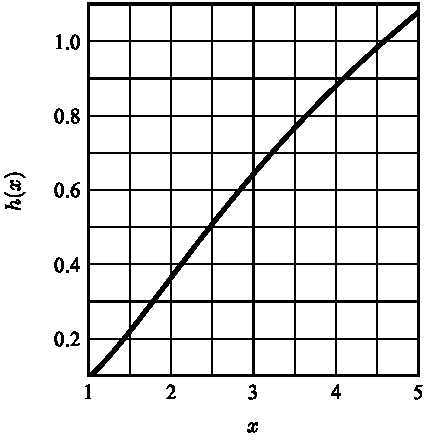
\includegraphics[width=7cm]{fig49.pdf}\\[0.3em]{\small 图 49}\end{minipage}\par\nopagebreak
我们在“常数”一词上加一个引号，是由于 $\kappa$ 实际上是某一与短程力性质有关的函数按小量 $ka$ 的幂展开后所得的首项.正如§133中指出的，低能共振相当于常数 $\kappa$ 特别小的情形.因而，为了改进精确度，我们必须计及这个展式中的下一项（$\sim k^2$），该项中含有一个数量级“正常”的系数，也就是必须把(138.12)式中的 $-\kappa$ 改成
\begin{equation*}
  -\kappa_0+\frac{1}{2}r_0k^2\,\text{\footnotemark}.
\end{equation*}
\footnotetext{对质子-质子散射，常数 $\alpha=1/\kappa_0$ 而 $r_0$ 的值为 $\alpha=-7.8\times10^{-13}$ cm，$r_0=2.8\times10^{-13}$ cm（库仑制长度单位为 $2\hbar^2/m_pe^2=57.6\times10^{-13}$ cm）.这些值是对自旋反平行的一对质子而言的：根据泡利原理，自旋平行的双质子系统不能处于 s 态.}
正如§133所说，共振的存在来自该系统的一个真的或虚的束缚态.可以证明\footnote{见 Л.~Ландау, Я.~Смородинский, ЖЭТФ, 14, 269, 1944.}，判断真能级或虚能级的判据仍然是常数 $\kappa$ 的符号.

根据(138.10)，波函数的总相移为 $\delta_l^{\text{库仑}}+\delta_l$，因而散射振幅为
\begin{equation}
  f(\theta)=\frac{1}{2\mathrm{i}k}\sum_{l=0}^{\infty}(2l+1)
  \left[\mathrm{e}^{2\mathrm{i}(\delta_l^{\text{库仑}}+\delta_l)}-1\right]
  \mathrm{P}_l(\cos\theta),
\end{equation}
方括号内的差可以写成
\begin{equation}
  \mathrm{e}^{2\mathrm{i}(\delta_l^{\text{库仑}}+\delta_l)}-1
  =\left[\mathrm{e}^{2\mathrm{i}\delta_l^{\text{库仑}}}-1\right]
  +\left[\mathrm{e}^{2\mathrm{i}\delta_l^{\text{库仑}}}
  \left(\mathrm{e}^{2\mathrm{i}\delta_l}-1\right)\right].
\end{equation}
库仑相移 $\delta_l^{\text{库仑}}$ 对所有的 $l$ 散射振幅给出数量级相同的贡献.相移 $\delta_l$ 和短程力有关，低能时 $l\neq0$ 的 $\delta_l$ 很小.因此，把(138.14)代入(138.13)时，每个求和项中保留(138.14)式的第一项，求和后即得库仑散射振幅(135.9)
\begin{equation}
  f_{\text{库仑}}(\theta)
  =-\frac{1}{2a_{\mathrm{c}}k^2\sin^2\dfrac{1}{2}\theta}
  \exp\left(-\frac{2\mathrm{i}}{ka_{\mathrm{c}}}
  \ln\sin\frac{1}{2}\theta
  +2\mathrm{i}\delta_0^{\text{库仑}}\right).
\end{equation}
(138.14)式中第二个括号只保留 $l=0$ 的项.因而总散射振幅为
\begin{equation}
  f(\theta)=f_{\text{库仑}}(\theta)
  +\frac{1}{2\mathrm{i}k}
  \left(\mathrm{e}^{2\mathrm{i}\delta_0}-1\right)
  \mathrm{e}^{2\mathrm{i}\delta_0^{\text{库仑}}}.
\end{equation}
上式中的第二项可以称为\textbf{核散射振幅}.但应强调指出，这种划分具有任意性：鉴于(138.11)中 $\delta_0$ 的定义，库仑作用的存在对 $\delta_0$ 这一项也有相当大的影响，这与不带电粒子短程力的相应项很不一样.特别是 $ka_{\mathrm{c}}\to0$ 时，相移 $\delta_0$ 以及(138.16)式中的第二项按 $\mathrm{e}^{-2\pi/ka_{\mathrm{c}}}$ 的规律指数式地趋于零.也就是说，核散射整个地被库仑斥力掩盖掉.

散射截面中，这两部分振幅是相干的：
\begin{equation}
\begin{aligned}
  \frac{\mathrm{d}\sigma}{\mathrm{d}o}=|f(\theta)|^2
  ={}&\left(\frac{Z_1Z_2e^2}{2mv^2}\right)^{2}
  \biggl[\frac{1}{\sin^4(\theta/2)}-\\
  &-\frac{4ka_{\mathrm{c}}}{\sin^2(\theta/2)}
  \sin\delta_0\cos\left(\frac{2}{ka_{\mathrm{c}}}\ln\sin\frac{\theta}{2}
  +\delta_0\right)
  +4(ka_{\mathrm{c}})^2\sin^2\delta_0\biggr].
\end{aligned}
\end{equation}
上式假定了相碰粒子是不同的，对同类粒子，散射振幅在取平方之前必须先对称化（参考§137）.

\section{快电子和原子的弹性碰撞}

快电子和原子的弹性碰撞可以用玻恩近似处理.只要入射电子的速度远大于原子中的电子速度即可.

由于电子和原子的质量差别很大，后者在碰撞中可以认为是不动的，质心为静止的坐标系就和原子为静止的坐标系重合.此时(126.7)式中的 $p$ 和 $p'$ 就代表碰撞前后的电子动量，$m$ 为电子质量，$\theta$ 角就是电子偏转角 $\vartheta$.(126.7)式中的势能 $U(r)$ 需要适当地定义.

§126中，我们计算了相对于碰撞前后自由粒子波函数而言的相互作用能的矩阵元 $U_{p'p}$.在和原子碰撞时，还应计及描述原子内部状态的波函数.弹性碰撞中，原子态保持不变.因此 $U_{p'p}$ 仍可作为由电子波函数 $\psi_p$ 和 $\psi_{p'}$ 所确定的矩阵元，它对原子波函数而言是对角的.换句话说，(126.7)式中的 $U(r)$ 应该取作对原子波函数平均以后的电子和原子间的相互作用势能.它等于 $e\varphi(r)$，其中的 $\varphi(r)$ 是原子中的平均电荷分布在 $r$ 点产生的势.

我们用 $\rho(r)$ 代表原子中的电荷密度分布，对势 $\varphi$ 而言，我们有以下泊松方程
\begin{equation*}
  \nabla^2\varphi=-4\pi\rho(\boldsymbol{r}).
\end{equation*}
所求的矩阵元 $U_{p'p}$ 基本上就是 $U$ 的（即 $\varphi$ 的）傅里叶分量（对应于波矢
$\boldsymbol{q}=\boldsymbol{k}'-\boldsymbol{k}$ 的傅里叶分量）.把泊松方程分别应用于每一个傅里叶分量，我们有
\begin{equation*}
  \nabla^2\left(\varphi_q\,\mathrm{e}^{\mathrm{i}q\cdot r}\right)
  =-q^2\varphi_q\,\mathrm{e}^{\mathrm{i}q\cdot r}
  =-4\pi\rho_q\,\mathrm{e}^{\mathrm{i}q\cdot r},
\end{equation*}
故
\begin{equation*}
  \varphi_q=4\pi\rho_q/q^2,
\end{equation*}
亦即
\begin{equation}
  \int\varphi\,\mathrm{e}^{-\mathrm{i}q\cdot r}\,\mathrm{d}V
  =\frac{4\pi}{q^2}\int\rho\,\mathrm{e}^{-\mathrm{i}q\cdot r}\,\mathrm{d}V.
\end{equation}
电荷密度 $\rho(\boldsymbol{r})$ 由电子电荷和核电荷所组成：
\begin{equation*}
  \rho=-en(r)+Ze\delta(\boldsymbol{r}),
\end{equation*}
式中 $en(r)$ 是原子中的电子电荷密度.乘以 $\mathrm{e}^{-\mathrm{i}q\cdot r}$ 并积分得
\begin{equation*}
  \int\rho\,\mathrm{e}^{-\mathrm{i}q\cdot r}\,\mathrm{d}V
  =-e\int n\,\mathrm{e}^{-\mathrm{i}q\cdot r}\,\mathrm{d}V+Ze.
\end{equation*}
由此得我们所关心的积分式
\begin{equation}
  \int U\,\mathrm{e}^{-\mathrm{i}q\cdot r}\,\mathrm{d}V
  =\frac{4\pi e^2}{q^2}\left[Z-F(q)\right],
\end{equation}
式中的 $F(q)$ 由下式定义：
\begin{equation}
  F(q)=\int n\,\mathrm{e}^{-\mathrm{i}q\cdot r}\,\mathrm{d}V
\end{equation}
并称为\textbf{原子形状因子}.它是散射角和入射电子速度的函数.

最后，把(139.2)代入(126.7)式，得快电子被原子弹性散射的截面公式\footnote{我们略去了进行散射的快电子和原子中电子间的交换作用，也就是没有把该系统的波函数对称化.这种做法的合理性是明显的：在“交换积分”中，自由粒子的急剧振荡波函数与原子中电子波函数之间的干涉效应，对散射振幅的贡献是很小的.}：
\begin{equation}
  \mathrm{d}\sigma=\frac{4m^2e^4}{\hbar^4q^4}
  \left[Z-F(q)\right]^2\mathrm{d}o,
  \qquad
  q=\frac{2mv}{\hbar}\sin\frac{1}{2}\vartheta.
\end{equation}
我们来考虑 $qa_0\ll1$ 的极限情形，$a_0$ 具有原子半径的数量级.小的散射角对应于小的 $q$：$\vartheta\ll v_0/v$，其中 $v_0\sim\hbar/ma_0$ 为原子中电子速度的数量级.

我们把 $F(q)$ 展成 $q$ 的幂级数.零级项为 $\int n\,\mathrm{d}V$，它是原子中的电子总数 $Z$.一级项和 $\int rn(r)\,\mathrm{d}V$ 成正比，也就是原子偶极矩的平均值；它恒等于零（见§75）.因此必须继续展开至二级项，得到
\begin{equation*}
  Z-F(q)=\frac{1}{6}q^2\int nr^2\,\mathrm{d}V;
\end{equation*}
代入(139.4)后得
\begin{equation}
  \mathrm{d}\sigma=\left|\frac{me^2}{3\hbar^2}
  \int nr^2\,\mathrm{d}V\right|^2\mathrm{d}o.
\end{equation}
由此可见，在小角度范围内，截面与散射角无关，并由原子中电子距离原子核的均方距离所给定.

在大 $q$（$qa_0\gg1$，即 $\vartheta\gg v_0/v$）的相反极限情形下，(139.3)被积函数中的 $\mathrm{e}^{-\mathrm{i}q\cdot r}$ 因子是一个急剧振荡函数，因而整个积分接近于零.和 $Z$ 相比我们就可以略去 $F(q)$，故
\begin{equation}
  \mathrm{d}\sigma=\left(\frac{Ze^2}{2mv^2}\right)^{2}
  \frac{\mathrm{d}o}{\sin^4\dfrac{1}{2}\vartheta},
\end{equation}
也就是说，我们得到原子核处的卢瑟福散射.

我们也能计算\textbf{输运截面}
\begin{equation}
  \sigma_{\mathrm{tr}}=\int(1-\cos\vartheta)\,\mathrm{d}\sigma.
\end{equation}
根据(139.5)式，在 $\vartheta\ll v_0/v$ 的角度范围内，我们有
$\mathrm{d}\sigma=$ 常数$\times\sin\vartheta\,\mathrm{d}\vartheta=$ 常数$\times\vartheta\,\mathrm{d}\vartheta$，式中的常数与 $\vartheta$ 无关.因此在这个范围内，上式积分中的被积函数和 $\vartheta^3$ 成正比，故在积分的下限很快地收敛.在 $1\gg\vartheta\gg v_0/v$ 的范围内，我们有 $\mathrm{d}\sigma\approx$ 常数$\times\mathrm{d}\vartheta/\vartheta^3$；被积函数与 $1/\vartheta$ 成正比，积分(139.7)对数性发散.由此可见，这个角度范围在积分中起着主要作用，我们只需对这个范围积分.积分的下限必须取 $v_0/v$ 的数量级；我们把它写成 $e^2/\gamma\hbar v$ 形式，$\gamma$ 是一个无量纲常数.结果得下列公式
\begin{equation}
  \sigma_{\mathrm{tr}}=4\pi\left(\frac{Ze^2}{mv^2}\right)^{2}
  \ln\frac{\gamma\hbar v}{e^2}.
\end{equation}
常数 $\gamma$ 的精确计算需要考虑 $\vartheta>v_0/v$ 的散射，无法表成一般形式.$\sigma_{\mathrm{tr}}$ 很少依赖于这个常数的选择，因为它只出现在对数之内，而且还乘上了一个很大的量 $\hbar v/e^2$.

为了对重原子的形状因子进行数值计算，我们可以采用托马斯—费米分布的密度 $n(r)$.我们知道，托马斯—费米模型中的 $n(r)$ 具有以下形式：
\begin{equation*}
  n(r)=Z^2f\left(\frac{rZ^{1/3}}{b}\right),
\end{equation*}
此式及以后各式中所有的量都用原子单位量度.很易看出，用这个函数 $n(r)$ 计算积分式(139.3)时，$q$ 只包含在组合 $qZ^{-1/3}$ 中：
\begin{equation}
  F(q)=Z\varphi(bqZ^{-1/3}).
\end{equation}
作为参考，表 11 给出了函数 $\varphi(x)$ 的值，它对所有的原子都成立\footnote{必须注意，这个式子对小的 $q$ 不能应用，因为此时 $nr^2$ 的积分实际上不能用托马斯-费米模型计算（见§113 的第 3 个注）.还须指出，托马斯-费米模型并不代表原子的个别性质以及它们随原子序的系统性变化.}.

\begin{center}
{\heiti 表 11}\quad 托马斯—费米模型的原子形状因子
\end{center}

\begin{center}
\begin{tabular}{|c|c||c|c||c|c|}
  \hline
  $x$ & $\varphi(x)$ & $x$ & $\varphi(x)$ & $x$ & $\varphi(x)$\\
  \hline
  $0$ & $1.000$ & $1.08$ & $0.422$ & $2.17$ & $0.224$\\
  $0.15$ & $0.922$ & $1.24$ & $0.378$ & $2.32$ & $0.205$\\
  $0.31$ & $0.796$ & $1.39$ & $0.342$ & $2.48$ & $0.189$\\
  $0.46$ & $0.684$ & $1.55$ & $0.309$ & $2.64$ & $0.175$\\
  $0.62$ & $0.589$ & $1.70$ & $0.284$ & $2.79$ & $0.167$\\
  $0.77$ & $0.522$ & $1.86$ & $0.264$ & $2.94$ & $0.156$\\
  $0.93$ & $0.469$ & $2.02$ & $0.240$ & & \\
  \hline
\end{tabular}
\end{center}

根据(139.9)的原子形状因子，截面(139.4)将呈以下形式：
\begin{equation}
\begin{aligned}
  \mathrm{d}\sigma
  =\frac{4Z^2}{q^4}\left[1-\varphi(bqZ^{-1/3})\right]^2\mathrm{d}o
  =Z^{2/3}\varPhi\left(Z^{-1/3}v\sin\frac{1}{2}\vartheta\right)
  \mathrm{d}o,
\end{aligned}
\end{equation}
其中的 $\varPhi(x)$ 是一个对所有原子都成立的新函数.总截面可经积分获得.由于小的 $\vartheta$ 角范围在这个积分中起主要作用，因此可以写成
\begin{equation*}
  \mathrm{d}\sigma\approx Z^{2/3}
  \varPhi(Z^{-1/3}v\vartheta/2)\,2\pi\vartheta\,\mathrm{d}\vartheta,
\end{equation*}
并把对 $\vartheta$ 的积分延伸至无穷大：
\begin{equation*}
  \sigma=2\pi Z^{2/3}\int_0^{\infty}
  \varPhi(Z^{-1/3}v\vartheta/2)\,\vartheta\,\mathrm{d}\vartheta
  =\frac{8\pi}{v^2}Z^{4/3}\int_0^{\infty}x\varPhi(x)\,\mathrm{d}x,
\end{equation*}
因此 $\sigma$ 的形式为
\begin{equation}
  \sigma=\text{常数}\times Z^{4/3}/v^2.
\end{equation}
同样，很易证明，(139.8)式中的 $\gamma$ 常数将与 $Z^{-1/3}$ 成正比.

\begin{xiti}

\noindent{\heiti 习题}\quad 计算快电子对基态氢原子的弹性散射截面.

解：氢原子基态波函数为（采用原子单位）$\psi=\mathrm{e}^{-r}/\sqrt{\pi}$，故
$n=\mathrm{e}^{-2r}/\pi$.(139.3)中对角度的积分与推导(126.12)式时相同.我们有
\begin{equation*}
  F=\frac{4\pi}{q}\int_0^{\infty}n(r)\sin qr\cdot r\,\mathrm{d}r
  =\frac{1}{\left(1+\dfrac{1}{4}q^2\right)^{2}},
\end{equation*}
代入(139.4)中得
\begin{equation*}
  \mathrm{d}\sigma=\frac{4(8+q^2)^2}{(4+q^2)^4}\,\mathrm{d}\sigma,
\end{equation*}
其中 $q=2v\sin\dfrac{1}{2}\vartheta$.令
$\mathrm{d}o=2\pi\sin\vartheta\,\mathrm{d}\vartheta=(2\pi/v^2)q\,\mathrm{d}q$
并对 $q$ 从0到 $2v$ 积分，可算出总截面；由于假定 $v$ 很大且积分收敛，积分上限可用无穷大代替，结果为
\begin{equation*}
  \sigma=\frac{7\pi}{3v^2}.
\end{equation*}
输运截面按下式计算：
\begin{equation*}
  \sigma_{\mathrm{tr}}=\frac{1}{2v^2}\int q^2\,\mathrm{d}\sigma.
\end{equation*}
改换积分变量，令 $u=4+q^2$，除 $\mathrm{d}u/u$ 这一项外积分上限均取无穷大，我们得
\begin{equation*}
  \sigma_{\mathrm{tr}}=\frac{4\pi}{v^4}
  \left(\ln v+\frac{1}{12}\right)
\end{equation*}
与(139.8)式一致.

\end{xiti}

\section{具有自旋轨道作用的散射}

迄今为止，我们只研究了粒子间相互作用与其自旋无关的碰撞.在这些条件下，自旋或者对散射过程根本没有影响，或者由于交换效应而只有间接影响（§137）.

现在来研究把§123中给出的散射理论推广到粒子间相互作用明显依赖于自旋的情形，这正是核粒子的碰撞中所发生的.

我们将详细讨论最简单的情形，其中一个相碰粒子的自旋为 $\dfrac{1}{2}$（为确定起见，把它取作入射粒子），另一个（靶粒子）的自旋为零.

对系统的一个给定角动量j（半整数），轨道角动量只能有 $l=j\pm\dfrac{1}{2}$ 两个值，它们对应于宇称不同的态.因此在这种情形下，轨道角动量绝对值的守恒来自j和宇称的守恒.

算符 $\hat{f}$（§125）现在不但作用在系统波函数的轨道变量上，而且也作用在它的自旋变量上.它应该和守恒量 $l^2$ 对易.这种算符的最一般形式为
\begin{equation}
  \hat{f}=\hat{a}+\hat{b}\,\hat{\boldsymbol{l}}\cdot\hat{\boldsymbol{s}},
\end{equation}
其中的 $\hat{a}$ 和 $\hat{b}$ 是轨道算符，只和 $l^2$ 有关.

S矩阵，从而还有算符 $\hat{f}$ 的矩阵，对于守恒量l和j（以及总角动量的分量m）具有定值的状态波函数而言是对角的，而且对角元可以通过(123.15)式用波函数的相位 $\delta$ 表达出来.对于给定的l和给定的总角动量 $j=l+\dfrac{1}{2}$ 或 $l-\dfrac{1}{2}$，$\boldsymbol{l}\cdot\boldsymbol{s}$ 的本征值分别为 $\dfrac{l}{2}$ 和 $-(l+1)/2$［见(118.5)］.因此，确定算符 $\hat{a}$ 和 $\hat{b}$ 的对角矩阵元（记作 $a_l$ 和 $b_l$）时，我们有关系式
\begin{equation}
\left.
\begin{aligned}
  &a_l+\frac{l}{2}b_l
  =\frac{1}{2\mathrm{i}k}
  \left(\mathrm{e}^{2\mathrm{i}\delta_l^{+}}-1\right),\\
  &a_l-\frac{l+1}{2}b_l
  =\frac{1}{2\mathrm{i}k}
  \left(\mathrm{e}^{2\mathrm{i}\delta_l^{-}}-1\right),
\end{aligned}
\right\}
\end{equation}
式中的相位 $\delta_l^{+}$ 和 $\delta_l^{-}$ 分别对应于 $j=l+\dfrac{1}{2}$ 和 $j=l-\dfrac{1}{2}$ 的态.

但是，我们感兴趣的并不在于算符 $\hat{f}$ 相对于给定l和j的态而言的那些对角元本身，而在于作为入射波方向和散射波方向的函数的散射振幅.这个振幅仍然是一个算符，但这只是针对自旋变量的，是对自旋分量 $\sigma$ 并不对角的一个算符.本节以后用记号 $\hat{f}$ 代表这个算符.

为了导出这个算符，我们必须把算符(140.1)作用在对应于入射平面波（沿 $z$ 轴）的函数(125.17)上.因而
\begin{equation}
  \hat{f}=\sum_{l=0}^{\infty}(2l+1)
  \left(a_l+b_l\,\hat{\boldsymbol{l}}\cdot\hat{\boldsymbol{s}}\right)
  \mathrm{P}_l(\cos\theta),
\end{equation}
式中还应算出算符 $\hat{\boldsymbol{l}}\cdot\hat{\boldsymbol{s}}$ 作用在 $\mathrm{P}_l(\cos\theta)$ 函数上的结果.它的做法是，先写出下式［见(29.11)］
\begin{equation*}
  \hat{\boldsymbol{l}}\cdot\hat{\boldsymbol{s}}
  =\frac{1}{2}\left(\hat{l}_{+}\hat{s}_{-}
  +\hat{l}_{-}\hat{s}_{+}\right)+\hat{l}_z\hat{s}_z,
\end{equation*}
再应用算符 $\hat{l}_{\pm}$ 的矩阵元公式(27.12)，或者更简单地应用算符表式(26.14)，(26.15)结果得
\begin{equation*}
  \hat{\boldsymbol{l}}\cdot\hat{\boldsymbol{s}}\,
  \mathrm{P}_l(\cos\theta)
  =\mathrm{i}\boldsymbol{\nu}\cdot\hat{\boldsymbol{s}}\,
  \mathrm{P}_l^{1}(\cos\theta),
\end{equation*}
式中的 $\mathrm{P}_l^1$ 是连带勒让德多项式，$\boldsymbol{\nu}$ 是一个垂直于散射平面的沿
$\boldsymbol{n}\times\boldsymbol{n}'$ 方向的单位矢量［$n$ 是入射（$z$ 轴）方向，$\boldsymbol{n}'$ 是由球极角 $\theta,\varphi$ 所定义的散射方向］.

由(140.2)式求出 $a_l$ 和 $b_l$ 后代入(140.3)式中，最后可得
\begin{equation}
  \hat{f}=A+2B\,\boldsymbol{\nu}\cdot\boldsymbol{s},
\end{equation}
\begin{equation}
\left.
\begin{aligned}
  &A=\frac{1}{2\mathrm{i}k}\sum_{l=0}^{\infty}
  \left[(l+1)\left(\mathrm{e}^{2\mathrm{i}\delta_l^{+}}-1\right)
  +l\left(\mathrm{e}^{2\mathrm{i}\delta_l^{-}}-1\right)\right]
  \mathrm{P}_l(\cos\theta),\\
  &B=\frac{1}{2k}\sum_{l=1}^{\infty}
  \left(\mathrm{e}^{2\mathrm{i}\delta_l^{+}}
  -\mathrm{e}^{2\mathrm{i}\delta_l^{-}}\right)
  \mathrm{P}_l^{1}(\cos\theta).
\end{aligned}
\right\}
\end{equation}
这个算符的矩阵元所给出的散射振幅，它的初末态具有确定的自旋投影值 $\sigma$ 和 $\sigma'$.我们来考虑对所有可能的 $\sigma'$ 值求和，并对初态中（入射束中）各种不同 $\sigma$ 的概率求平均以后的截面.这样的截面由下式给出：
\begin{equation}
  \mathrm{d}\sigma=\overline{\left(f^{+}f\right)_{\sigma\sigma}}\,
  \mathrm{d}o;
\end{equation}
乘积 $\hat{f}^{+}\hat{f}$ 取对角矩阵元相当于对末态求和\footnote{设 $|f_{0n}|^2$ 为某一算符的 $0\to n$ 跃迁矩阵元的模量平方，对末态 $n$ 求和后，我们有
\begin{equation*}
  \sum_n|f_{0n}|^2=\sum_n f_{0n}(f_{0n})^{*}
  =\sum_n f_{0n}(f^{+})_{n0}=(ff^{+})_{00}.
\end{equation*}
为避免误解，我们必须指出，(140.6)中的 $^{+}$ 号代表 $\hat{f}$（自旋的算符）的厄米共轭，并不是 $\boldsymbol{n}$ 和 $\boldsymbol{n}'$ 的转置.}，横线则代表对初态求平均.如果初态中所有的自旋方向都是等概率的，这个平均就可以化成取矩阵的阵迹除以自旋分量 $\sigma$ 的可能值的个数：
\begin{equation}
  \mathrm{d}\sigma=\frac{1}{2}\mathrm{tr}\left(f^{+}f\right)
  \mathrm{d}o
\end{equation}
把(140.4)代入(140.6)后，$(\boldsymbol{\nu}\cdot\boldsymbol{s})^2$ 的平均值可按
$\dfrac{1}{3}\nu^2s^2=\dfrac{1}{3}s(s+1)=\dfrac{1}{4}$ 算出，结果得
\begin{equation}
  \frac{\mathrm{d}\sigma}{\mathrm{d}o}=|A|^2+|B|^2
  +2\,\mathrm{Re}\left(AB^{*}\right)\boldsymbol{\nu}\cdot\boldsymbol{P},
\end{equation}
式中的 $\boldsymbol{P}=2\bar{\boldsymbol{s}}$ 是入射束的初始极化度，它的定义是初态中的自旋平均值和其最大可能值 $\left(\dfrac{1}{2}\right)$ 之比.在自旋为 $\dfrac{1}{2}$ 情形下，矢量 $\boldsymbol{P}$ 完全描述了自旋态（§59）.

可以指出的是，入射束的极化导致了散射的方位角不对称性：因为截面式(140.8)中的最后一项 $\boldsymbol{\nu}\cdot\boldsymbol{P}$ 不但和极角 $\theta$ 有关而且和矢量 $\boldsymbol{n}'$ 相对于 $n$ 的方位角 $\varphi$ 有关（如果极化不垂直于 $\boldsymbol{\nu}$，则
$\boldsymbol{\nu}\cdot\boldsymbol{P}\neq0$）.

散射粒子的极化度可从下式算出：
\begin{equation}
  P'=\frac{2\left(f^{+}sf\right)_{\sigma\sigma}}
  {\left(f^{+}f\right)_{\sigma\sigma}}.
\end{equation}
如果初态是非极化的（$\boldsymbol{P}=0$），经简单计算给出
\begin{equation}
  P'=\frac{2\,\mathrm{Re}(AB^{*})}{|A|^2+|B|^2}\,\boldsymbol{\nu}.
\end{equation}
可见一般讲来，散射会导致垂直于散射平面的极化.可是，这种效应在玻恩近似中并不存在：如果所有的相位 $\delta$ 都很小，系数 $A$ 在相移的一级近似下是一个实量，而 $B$ 是一个纯虚量，故
\begin{equation*}
  \mathrm{Re}\left(AB^{*}\right)=0.
\end{equation*}
(140.10)的极化 $\boldsymbol{P}'$ 沿着 $\boldsymbol{\nu}$ 方向这一点是显然的：$\boldsymbol{P}'$ 是一个轴矢量，而 $\boldsymbol{\nu}$ 是现有的极矢量 $n$ 和 $\boldsymbol{n}'$ 所能组成的唯一的轴矢量.因此很明显，自旋为 $\dfrac{1}{2}$ 的非极化粒子束，被自旋为任意的（不一定为零）原子核所组成的非极化靶\footnote{这里指的是自旋方向完全任意分布的靶.记得 $s>\frac{1}{2}$ 时，自旋矢量的平均值并不完全确定自旋态，当这个平均值等于零时不一定意味着自旋的完全无序.}散射时，散射粒子的极化也将具有这个性质.

表述散射的倒易定理时应该记得，时间反演不但使动量变号而且还使角动量变号，因此在具有自旋的情形下，散射的时间反演对称性必须表现为下述两个过程的振幅相等，这两个过程的差别不只是初末态的对调以及运动方向的反号，而且还有这两个态中粒子自旋分量的反号.此外，这两个振幅的符号有可能不同，因为根据(60.3)式，时间反演会在自旋波函数中引进一个
$(-1)^{s-\sigma}$ 因子.结果使倒易定理表成以下形式\footnote{此式的推导类似于(125.12).入射波和出射波的振幅中必须含有自旋因子，(125.10)式应改为条件 $\hat{K}^{-1}\tilde{\hat{S}}\hat{K}=\tilde{\hat{S}}$，其中算符 $\hat{K}$ 不但进行反演而且还按(60.3)式改变自旋态.}：
\begin{equation}
\begin{aligned}
  &f(\sigma_1,\sigma_2,\boldsymbol{n};
  \sigma_1',\sigma_2',\boldsymbol{n}')\\
  &\qquad=(-1)^{\sum(s-\sigma)}
  f(-\sigma_1',-\sigma_2',-\boldsymbol{n}';
  -\sigma_1,-\sigma_2,-\boldsymbol{n}),
\end{aligned}
\end{equation}
式中的
$f(\sigma_1,\sigma_2,\boldsymbol{n};\sigma_1',\sigma_2',\boldsymbol{n}')$
是使碰撞粒子的自旋分量由 $\sigma_1,\sigma_2$ 变到 $\sigma_1',\sigma_2'$ 的散射振幅.指数中的求和是取遍散射前后的粒子.

玻恩近似中，散射具有进一步的对称性，初末态对调但粒子动量和自旋分量不像时间反演那样变号的两个过程，它们的概率相同（见§126）.把这个性质和倒易定理联合起来，我们发现，散射对动量和自旋分量的全部反号（但不对调）具有对称性.从而很易得出结论，在玻恩近似中，任何非极化粒子束对非极化靶的散射不会有极化效应.因为在上述变换下，极化矢量 $\boldsymbol{P}$ 变号，应该和 $\boldsymbol{P}$ 同向的单位矢量
$\boldsymbol{k}\times\boldsymbol{k}'$ 却不变号.由此可知，上述自旋为 $\dfrac{1}{2}$ 的粒子对零自旋粒子散射的有关性质，实际上是一个普遍性质.

当碰撞粒子的自旋为任意时，角分布的一般公式极为复杂，我们不在这里推导，只是计算一下确定这种角分布所需的参量数.

前面考虑过自旋为 $\dfrac{1}{2}$ 和0的两个粒子的碰撞情形，它具有这样的性质，当j和宇称给定以后，此双粒子系统只能有一个态（不计总角动量空间取向这一不重要的方面）.每一个这样的态在散射振幅中导致一个实参量（相位 $\delta$）.对于其它的自旋，一般讲来会有几个不同的态具有相同的总角动量J和相同的宇称，这些态由总自旋S和粒子间的相对运动轨道角动量l的数值相区别.假定这些态的数目为n，很易看出，每一组这样的态在散射振幅中提供 $\dfrac{1}{2}n(n+1)$ 个实参量.这是因为，对这组态而言，S矩阵是一个具有幺正对称性的矩阵（由于倒易定理），它有 $n\times n$ 个复矩阵元.这个矩阵中的独立参量数是很易算出的，只要注意到，如果把算符 $\hat{S}$ 写成 $\hat{S}=\exp(\mathrm{i}\hat{R})$ 的形式，当 $\hat{R}$ 为任一厄米算符时，$\hat{S}$ 的幺正性就自动得到满足［见(12.13)］.如果 $\hat{S}$ 是对称的，则矩阵 $\hat{R}$ 也是，但 $\hat{R}$ 是厄米的，故它必是实的，而一个实对称矩阵具有 $\dfrac{1}{2}n(n+1)$ 个独立分量.

以自旋为 $\dfrac{1}{2}$ 的两个粒子为例，数 $n=2$，J给定后共有四个态：两个态的 $l=J$ 而总自旋 $S=0$ 或1；另两个态的 $l=J\pm1$，$S=1$.显然，其中两个是偶态（l偶数），两个是奇态（l奇数）.

两个自旋为 $\dfrac{1}{2}$ 的粒子的散射振幅，作为和这两个粒子的自旋变量有关的一个算符，根据必要的不变性条件（时间反演下必须是一个不变的标量），很易写出它的一般表式.为了构造出这个表式，我们一共有两个粒子的自旋轴矢量 $\boldsymbol{s}_1$ 和 $\boldsymbol{s}_2$ 以及两个普通（极）矢量 $n$ 和 $\boldsymbol{n}'$ 可供我们支配.每个 $\hat{\boldsymbol{s}}_1$ 和 $\hat{\boldsymbol{s}}_2$ 算符在振幅中一定呈线性，因为自旋为 $\dfrac{1}{2}$ 的算符的任意函数总能化成线性函数.满足这些条件的算符的最普遍的形式可以写成
\begin{equation}
\begin{aligned}
  \hat{f}={}&A+B\left(\hat{\boldsymbol{s}}_1\cdot\boldsymbol{\lambda}\right)
  \left(\hat{\boldsymbol{s}}_2\cdot\boldsymbol{\lambda}\right)
  +C\left(\hat{\boldsymbol{s}}_1\cdot\boldsymbol{\mu}\right)
  \left(\hat{\boldsymbol{s}}_2\cdot\boldsymbol{\mu}\right)+\\
  &+D\left(\hat{\boldsymbol{s}}_1\cdot\boldsymbol{\nu}\right)
  \left(\hat{\boldsymbol{s}}_2\cdot\boldsymbol{\nu}\right)
  +E\left(\hat{\boldsymbol{s}}_1+\hat{\boldsymbol{s}}_2\right)\cdot\boldsymbol{\nu}
  +F\left(\hat{\boldsymbol{s}}_1-\hat{\boldsymbol{s}}_2\right)\cdot\boldsymbol{\nu}.
\end{aligned}
\end{equation}
系数 $A,B,\cdots$ 都是些标量，它们仅和标量 $\boldsymbol{n}\cdot\boldsymbol{n}'$ 有关，亦即和散射角 $\theta$（以及和能量）有关；$\boldsymbol{\lambda},\boldsymbol{\mu},\boldsymbol{\nu}$ 分别为沿
$\boldsymbol{n}+\boldsymbol{n}'$，$\boldsymbol{n}-\boldsymbol{n}'$ 和
$\boldsymbol{n}\times\boldsymbol{n}'$ 方向的三个相互垂直的单位矢量.时间反演操作相当于作以下变换：
\begin{equation*}
  \boldsymbol{s}_1\to-\boldsymbol{s}_1,\qquad
  \boldsymbol{s}_2\to-\boldsymbol{s}_2,\qquad
  \boldsymbol{n}\to-\boldsymbol{n}',\qquad
  \boldsymbol{n}'\to-\boldsymbol{n},
\end{equation*}
从而有
\begin{equation*}
  \boldsymbol{\lambda}\to-\boldsymbol{\lambda},\qquad
  \boldsymbol{\mu}\to\boldsymbol{\mu},\qquad
  \boldsymbol{\nu}\to-\boldsymbol{\nu}.
\end{equation*}
算符(140.12)的不变性很明显.

核子（质子和中子）的相互散射中，(140.12)的最后一项并不出现.这是因为核子间的核力不改变系统的总自旋值S，可是算符
$\hat{\boldsymbol{s}}_1-\hat{\boldsymbol{s}}_2$ 并不和 $\hat{S}^2$ 对易（根据(117.4)式，(140.12)中其余项可用总自旋算符 $\hat{\boldsymbol{s}}$ 表出，因此和算符 $\hat{S}^2$ 对易）.同类核子（pp或nn）的散射中，系数 $A,B,\cdots$ 作为散射角的函数还满足某些对称关系，这是两个粒子全同的结果（见题2）.

\begin{xiti}

\noindent{\heiti 习题1}\quad 自旋为 $\dfrac{1}{2}$ 的粒子被自旋为零的粒子所散射，如果散射前极化不等于零，求散射后的极化.

解：计算(140.9)式时最好取其分量式，令 $z$ 轴沿 $\boldsymbol{\nu}$ 方向.结果为
\begin{equation*}
  P'=\frac{\left(|A|^2-|B|^2\right)\boldsymbol{P}
  +2|B|^2\,\boldsymbol{\nu}\left(\boldsymbol{\nu}\cdot\boldsymbol{P}\right)
  +2\,\mathrm{Im}\left(AB^{*}\right)\boldsymbol{\nu}\times\boldsymbol{P}
  +2\,\mathrm{Re}\left(AB^{*}\right)\boldsymbol{\nu}}
  {|A|^2+|B|^2+2\,\mathrm{Re}\left(AB^{*}\right)
  \boldsymbol{\nu}\cdot\boldsymbol{P}}.
\end{equation*}

\noindent{\heiti 习题2}\quad 试求两个相同核子的散射振幅中系数（作为 $\theta$ 角的函数）所应满足的对称条件（R.~Oehme，1955）.

解：我们把(140.12)中的各项重新分组，使得每组仅当双核子系统的态为单态（S=0）或三重态（S=1）时才不为零：
\setcounter{equation}{0}\renewcommand{\theequation}{\arabic{equation}}%
\begin{equation}
\begin{aligned}
  \hat{f}={}&a\left(\hat{\boldsymbol{s}}_1\cdot\hat{\boldsymbol{s}}_2
  -\frac{1}{4}\right)
  +b\left(\hat{\boldsymbol{s}}_1\cdot\hat{\boldsymbol{s}}_2
  +\frac{3}{4}\right)
  +c\left[\frac{1}{4}
  +\left(\hat{\boldsymbol{s}}_1\cdot\boldsymbol{\nu}\right)
  \left(\hat{\boldsymbol{s}}_2\cdot\boldsymbol{\nu}\right)\right]+\\
  &+d\left[\left(\hat{\boldsymbol{s}}_1\cdot\boldsymbol{n}\right)
  \left(\hat{\boldsymbol{s}}_2\cdot\boldsymbol{n}'\right)
  +\left(\hat{\boldsymbol{s}}_1\cdot\boldsymbol{n}'\right)
  \left(\hat{\boldsymbol{s}}_2\cdot\boldsymbol{n}\right)\right]
  +e\left(\hat{\boldsymbol{s}}_1+\hat{\boldsymbol{s}}_2\right)
  \cdot\boldsymbol{\nu}.
\end{aligned}
\end{equation}
应用(117.4)式，很易看出第一项仅当S=0时才不等于零，其余项仅当S=1时才不等于零.由于粒子的全同性，散射振幅对粒子坐标的交换当S=0时必须是对称的，S=1时必须是反对称的.这种变换等价于 $\theta\to\pi-\theta$，或者是把矢量 $\boldsymbol{n}$ 和 $\boldsymbol{n}'$ 中的一个变号（参考§137）.根据这些条件，我们得到以下关系：
\begin{equation}
\left.
\begin{aligned}
  &a(\pi-\theta)=a(\theta),\qquad
  b(\pi-\theta)=-b(\theta),\qquad
  c(\pi-\theta)=-c(\theta),\\
  &d(\pi-\theta)=d(\theta),\qquad
  e(\pi-\theta)=e(\theta).
\end{aligned}
\right\}
\end{equation}
由于同位旋守恒，nn 和 pp 散射以及同位旋态 $T=1$ 的np 散射具有相同的散射振幅.但对np系统还可有 $T=0$ 的态，因此np散射振幅要用不同于(1)式的系数 $a,b,\cdots$ 来描写，这些系数并不具备(2)式的对称性质.

\end{xiti}
\setcounter{equation}{0}\renewcommand{\theequation}{\arabic{section}.\arabic{equation}}%

\section{雷杰极点}

在§128中，我们把散射振幅看作粒子能量 $E$ 的复变函数研究了它的解析性质，轨道角动量l作为一个参量具有实的整数值.如果现在针对实的能量值E把l看作一个连续的复变量，那么从方法论意义上来看，散射振幅将会进一步呈现一些十分重要的性质\footnote{这些性质首先由雷杰（T.~Regge，1958）进行了研究.}.

和§128一样，我们取具有以下渐近式的径向波函数：
\begin{equation}
  \chi_l=rR_l=A(l,E)
  \exp\left(-\frac{\sqrt{-2mE}}{\hbar}\,r\right)
  +B(l,E)\exp\left(\frac{\sqrt{-2mE}}{\hbar}\,r\right).
\end{equation}
这些函数是薛定谔方程(32.8)之解（式中的l现在看作复变量），同时，我们按以下条件从两个独立解中选择一个：
\begin{equation}
  \text{当}\ r\to0\ \text{时},\quad R_l\approx\text{常数}\times r^{l}.
\end{equation}
可以立刻看出，这个条件对参量l的允许值给予了一定的限制.实际上，$r$ 很小时，(32.8)式之解的一般形式为（见§32末）
\begin{equation*}
  R_l\approx c_1r^l+c_2r^{-l-1}.
\end{equation*}
为了使第二个解明显区别于第一个解并把它去掉，$r^{-l-1}$ 项当 $r\to0$ 时必须超过 $r^l$ 项.对于复的l，这一点导致 $\mathrm{Re}\,l>\mathrm{Re}(-l-1)$，或
\begin{equation}
  \mathrm{Re}\left(l+\frac{1}{2}\right)>0.
\end{equation}
以后我们只考虑垂直线 $l=-\dfrac{1}{2}$ 右边的那一半l复平面.

波函数 $R(r;l,E)$ 为系数对l解析的一个微分方程之解，它是l的一个解析函数，在半平面(141.3)内没有奇点.这一点特别适用于渐近式(141.1)，因而函数 $A(l,E)$ 和 $B(l,E)$ 对l没有奇点.可是，在这里已经假定了 $r\to\infty$ 时(141.1)中的两项都给保留是合理的.这一点当 $E>0$ 时总是对的，当 $E<0$ 时，如果场 $U(r)$ 满足条件(128.6)或(128.13)，这一点也是对的.这些论断中重要的是波函数渐近行为（对r）的方式依赖于E而不依赖于l.因此它的趋于这个渐近式并不受l为复数这一事实的影响.

比较(141.1)和渐近式(128.15)，我们发现S矩阵元呈以下形式：
\begin{equation}
  S(l,E)=\exp\left[2\mathrm{i}\delta(l,E)\right]
  =\mathrm{e}^{\mathrm{i}\pi l}\frac{A(l,E)}{B(l,E)},
\end{equation}
此式对复的l也成立（尽管“相移” $\delta$ 此时不再是实的）.

对于实的l和 $E>0$，函数A和B有(128.4)式的关系：
$A(l,E)=B^{*}(l,E)$.因而对复的l有
\begin{equation}
  A(l^{*},E)=B^{*}(l,E),\qquad E>0.
\end{equation}
从而 $S(l,E)$ 满足复幺正条件：
\begin{equation}
  S^{*}(l,E)\,S(l^{*},E)=1.
\end{equation}
由于 $A(l,E)$ 和 $B(l,E)$ 作为l的函数没有奇点，因此函数 $S(l,E)$ 以及分波振幅 $f(l,E)$ 只在函数 $B(l,E)$ 的零点处具有奇点（极点）.散射振幅在l复平面中的这些极点称为\textbf{雷杰极点}.它们的位置当然依赖于实参量E的值.确定极点位置的函数
\begin{equation*}
  l=\alpha_i(E)
\end{equation*}
称为\textbf{雷杰轨迹}.当E变动时，极点在l面内沿一定的曲线运动.下标i是极点的编号，以后将略去.

现在研究雷杰轨迹的性质，我们先来证明 $E<0$ 时所有的 $\alpha(E)$ 都是实函数.为此，我们考虑以下方程：
\begin{equation}
  \chi''+\left[\frac{2m}{\hbar^2}\left(E-U(r)\right)
  -\frac{\alpha(\alpha+1)}{r^2}\right]\chi=0,
\end{equation}
这是 $l=\alpha$ 的波函数所应满足的方程.此式乘 $\chi^{*}$ 并对r积分（第一项作分部积分），得到
\begin{equation*}
  -\int_0^{\infty}|\chi'|^2\,\mathrm{d}r
  +\frac{2m}{\hbar^2}\int_0^{\infty}(E-U)|\chi|^2\,\mathrm{d}r
  -\alpha(\alpha+1)\int_0^{\infty}\frac{|\chi|^2}{r^2}\,\mathrm{d}r=0.
\end{equation*}
式中应用了 $B=0$ 时（确定雷杰极点的条件）波函数在 $r\to\infty$ 过程中指数衰减的事实，所以各个积分都是收敛的.上式前两项是实的，所以最后一项的积分也是实的.从而必须有
\begin{equation*}
  \mathrm{Im}\left[\alpha(\alpha+1)\right]
  =\mathrm{Im}\left(\alpha+\frac{1}{2}\right)^{2}
  =2\,\mathrm{Re}\left(\alpha+\frac{1}{2}\right)\mathrm{Im}\,\alpha=0.
\end{equation*}
但是我们考虑的只是半平面(141.3)内的极点，肯定地有
\begin{equation*}
  \mathrm{Re}\left(\alpha+\frac{1}{2}\right)>0,
\end{equation*}
这就给出了所求的结果：
\begin{equation}
  \mathrm{Im}\,\alpha(E)=0\qquad(E<0\ \text{时}).
\end{equation}
其次，我们对(141.7)式进行和推导(128.10)式一样的手续：对E微分后乘以 $\chi$，减去乘 $\partial\chi/\partial E$ 的(141.7)式，得到以下恒等式：
\begin{equation*}
  \left[\chi'\frac{\partial\chi}{\partial E}
  -\chi\left(\frac{\partial\chi}{\partial E}\right)'\right]'
  -\frac{2m}{\hbar^2}\chi^2
  +\frac{\chi^2}{r^2}\frac{\mathrm{d}\alpha(\alpha+1)}{\mathrm{d}E}=0,
\end{equation*}
上式对r从0到 $\infty$ 积分，再利用 $r\to\infty$ 时 $\chi\to0$ 的事实，可证上式第一项的积分等于零，于是有
\begin{equation}
  \frac{\mathrm{d}\alpha(\alpha+1)}{\mathrm{d}E}
  \int_0^{\infty}\frac{\chi^2}{r^2}\,\mathrm{d}r
  =\frac{2m}{\hbar^2}\int_0^{\infty}\chi^2\,\mathrm{d}r.
\end{equation}
我们已知 $\alpha$ 是实的，波函数也是实的，因而(141.9)中的两个积分都是正的.故
\begin{equation*}
  \frac{\mathrm{d}}{\mathrm{d}E}\alpha(\alpha+1)
  =2\left(\alpha+\frac{1}{2}\right)\frac{\mathrm{d}\alpha}{\mathrm{d}E}>0
\end{equation*}
又由于 $\alpha+\dfrac{1}{2}>0$，故得
\begin{equation*}
  \frac{\mathrm{d}\alpha}{\mathrm{d}E}>0
  \qquad(E<0\ \text{时}).
\end{equation*}
可见 $E<0$ 时函数 $\alpha(E)$ 随E单调地增长.

函数 $\alpha(E)$ 取“物理”值时（即取 $l=0,1,2,\cdots$ 整数值时），所得的负E值对应于该系统的离散能级.我们注意到，这一点给出了根据它们所在的雷杰轨迹对束缚态进行分类的一个新原则.

作为一个例子，我们考虑在库仑引力场中运动的雷杰轨迹.此时散射矩阵元为\footnote{参考(135.11)式，该式中的 $k$ 必须变号以便把斥力改为引力.}
\begin{equation}
  S_l=\frac{\Gamma\left(l+1-\mathrm{i}/k\right)}
  {\Gamma\left(l+1+\mathrm{i}/k\right)},
\end{equation}
k用库仑单位.此式的极点是 $\Gamma(l+1-\mathrm{i}/k)$ 的宗量为负整数或零的那些点.$E<0$ 时 $k=\mathrm{i}\sqrt{-2E}$，故
\begin{equation}
  \alpha(E)=-n_r-1+\frac{1}{\sqrt{-2E}},
  \qquad E<0,
\end{equation}
其中 $n_r=0,1,2,\cdots$ 是雷杰轨迹的编号.令 $\alpha(E)$ 等于 $l=0,1,2,\cdots$ 中的一个整数，我们得到熟知的库仑场中离散能级的玻尔公式：
\begin{equation*}
  E=-\frac{1}{2}\left(n_r+1+l\right)^{-2}.
\end{equation*}
$n_r$ 在这里与确定径向波函数节点数的径量子数相一致，每条雷杰轨迹（即对每个给定的 $n_r$ 值）对应于无穷多个轨道角动量值不同的能级.

现在来考虑 $E>0$ 时 $\alpha(E)$ 函数的性质.(141.1)式中复变量E的函数 $A(l,E)$ 和 $B(l,E)$ 是定义在以右实轴为割线的一个平面上的（见§128）.与此相应，使 $B(l,E)=0$ 的函数 $l=\alpha(E)$ 具有同样的割线.在割线的上下沿，$\alpha(E)$ 具有复共轭值，在上沿有 $\mathrm{Im}\,\alpha>0$.对此我们不准备停留在只作形式上的证明，而要对其原因作出更为物理的解释.

当l为复数时，离心能以及有效势能
$U_l=U+l(l+1)/(2mr^2)$ 也成为复数.重复§19中的推导，(19.6)式现在改为
\begin{equation*}
  \frac{\partial}{\partial t}|\psi|^2+\nabla\cdot\boldsymbol{j}
  =2|\psi|^2\,\mathrm{Im}\,U_l.
\end{equation*}
当 $l=\alpha$ 和 $\mathrm{Im}\,\alpha>0$ 时，我们还有 $\mathrm{Im}\,U_l>0$.于是上式右边是正的，这表示场体积内辐射一个新粒子.因此波函数的渐近式（当 $B=0$ 时，只含(141.1)中的第一项）必须表为出射波，这发生在割线的上沿（参考从(128.1)到(128.3)式的推导）.

由于 $E>0$ 时 $\alpha(E)$ 是复函数，它不能取“物理”值 $l=0,1,2,\cdots$.可是，它有可能在l复平面上接近于这些值.我们来证明，这就会在分波振幅中出现共振（对应于所考虑的l的整数值）.

设 $l_0$ 为接近于函数 $\alpha(E)$ 的整数值，并令 $E_0$ 为
$\mathrm{Re}\,\alpha(E_0)=l_0$ 时的能量值（实的和正的）.于是在此值附近，我们有
\begin{equation}
  \alpha(E)\approx l_0+\mathrm{i}\eta+\beta(E-E_0),
\end{equation}
其中 $\eta=\mathrm{Im}\,\alpha(E_0)$ 是一个实常数.我们将考虑割线上沿的 $\alpha(E)$ 值.按照前面的讨论，这种情形下 $\eta>0$（并且有 $\eta\ll1$，根据 $\alpha$ 接近于 $l_0$ 的假定）.很易看出，常数 $\beta$（即 $E=E_0$ 处的导数 $\mathrm{d}\alpha/\mathrm{d}E$）可以看作是实的和正的.实际上，由于 $\alpha(E)$ 差不多是实的，所以波函数 $\chi(r;\alpha,E)$ 也差不多是实的.略去 $\eta$ 的高级小量后，我们可以略去 $\chi$ 的虚部，从而 $\beta$ 是正的，因为(141.9)中的积分是正的\footnote{为了阐明这些积分的结构，我们注意 $r\gg a$ 的渐近区（$a$ 是场的作用范围）内波函数的(141.1)式是成立的，当 $\eta$ 很小时，此区对积分式只有很小的贡献.事实上，如果 $l=\alpha(E)$ 是 $B(l,E)$ 的一个零点，则按(141.5) $l=\alpha^{*}$ 是 $A(l,E)$ 的一个零点.因此 $A(\alpha,E)$ 从而 $\chi(r;\alpha,E)$ 在 $r\gg a$ 区内都是一些小量 $\sim\eta^{1/2}$，见(134.11).估计这些积分时，还有一个重要之点是，在割线的上沿（对 $E$ 的关系），波函数含有一个因子
\begin{equation*}
  \mathrm{e}^{\mathrm{i}kr}\colon\ \chi(r;\alpha,E)=A(\alpha,E)\mathrm{e}^{\mathrm{i}kr}.
\end{equation*}
在这个上沿，$E$ 可看作 $E+\mathrm{i}\delta$（$\delta\to+0$）；则 $k$ 也有一个小的正虚部，它保证了(141.9)式中积分的收敛性.从物理上讲，$r\gg a$ 区对积分的贡献所以小，是由于能量 $E_0$ 对应于一个准定态（见后）；粒子到达此区只能是该态的一个罕有衰变的结果.积分的主要贡献来自 $r\sim a$ 区，在此区内波函数差不多是实的.}.

由于 $l=\alpha(E)$ 是 $B(l,E)$ 的一个零点，后者在 $\alpha,E_0$ 点附近正比于 $\alpha-l$.应用(141.12)，我们就有
\begin{equation}
  B(l_0,E)\approx\text{常数}\times
  \left[a(E-E_0)+\mathrm{i}\eta\right].
\end{equation}
此式的形状与(134.6)式相同，该式中的 $E_0$ 是能量，$\Gamma=2\eta/a>0$ 是准离散能级的宽度.由此可见，雷杰轨迹（$E>0$）对l整数值的接近对应于该系统的准定态.因此对这些态来讲存在着与严格定态一样的分类原则：每条雷杰轨迹可以对应于一族离散的和准离散的能级.

把l处理成为复变量使我们有可能导出总散射振幅（对 $E>0$）的一个有用积分形式，它可由级数(123.11)得出
\begin{equation}
  f(\mu)=\frac{1}{2\mathrm{i}k}\sum_{l=0}^{\infty}(2l+1)
  \left[S(l,E)-1\right]\mathrm{P}_l(\mu),
  \qquad\mu=\cos\theta.
\end{equation}
为此，首先不但须对 $l\geqslant0$ 的整数而且也应对所有的复值l定义出函数 $\mathrm{P}_l(\mu)$.这一点可把 $\mathrm{P}_l(\mu)$ 看作方程(c.2)之解来实现：
\begin{equation}
  \left(1-\mu^2\right)\mathrm{P}''_l(\mu)
  -2\mu\,\mathrm{P}'_l(\mu)
  +l(l+1)\mathrm{P}_l(\mu)=0.
\end{equation}
其边界条件为 $\mathrm{P}_l(1)=1$.这样定义的 $\mathrm{P}_l(\mu)$，作为l的函数对有限的l值没有奇点\footnote{把(141.15)和(e.2)比较，我们可把 $\mathrm{P}_l(\mu)$ 表成超几何函数
\begin{equation*}
  \mathrm{P}_l(\mu)=\mathrm{F}\left(-l,l+1,1;\frac{1}{2}-\frac{1}{2}\mu\right)
\end{equation*}}.

很易证明级数(141.14)等于下列积分
\begin{equation}
  f(\mu)=\frac{1}{4k}\int_{C}
  \frac{2l+1}{\sin\pi l}
  \left[S(l,E)-1\right]\mathrm{P}_l(-\mu)\,\mathrm{d}l,
\end{equation}
式中积分回线 $C$ 沿负向（顺时针方向）绕实轴上所有 $l=0,1,2,\cdots$ 诸点并在无穷远处封闭.

函数 $S(l,E)$ 的所有极点 $l=\alpha_1,\alpha_2,\cdots$（$E>0$ 时不在实轴上）必须留在回线 $C$ 的外面.积分(141.16)可化成 $-2\pi\mathrm{i}$ 乘以被积函数在 $l=0,1,2,\cdots$ 诸点的留数之和，$l=0,1,2,\cdots$ 是函数 $1/\sin\pi l$ 的极点，其留数为 $(-1)^l/\pi$.由于对整数l有
$\mathrm{P}_l(-\mu)=(-1)^l\mathrm{P}_l(\mu)$，我们就从(141.16)得到(141.14)式\footnote{本节所讨论的概念（非相对论理论）在§123 所引的 de~Alfaro, Regge 的书中给出了详细论述.}.

\begin{xiti}

\noindent{\heiti 习题}\quad 证明对应于一系列角动量l的相移满足不等式
\begin{equation*}
  \delta_{l+1}(E)-\delta_l(E)<\pi/2.
\end{equation*}
解：我们把l看成连续的实变量，并对(32.10)式进行微分
\begin{equation*}
  \frac{\partial\chi''}{\partial l}
  +\left[\frac{2m}{\hbar^2}(E-U)
  -\frac{l(l+1)}{r^2}\right]\frac{\partial\chi}{\partial l}
  =(2l+1)\frac{\chi}{r^2}.
\end{equation*}
将此式乘以 $\chi$，并将原式乘以 $\partial\chi/\partial l$，两式相减得
\begin{equation*}
  \left[\chi\frac{\partial\chi'}{\partial l}
  -\chi'\frac{\partial\chi}{\partial l}\right]'
  =(2l+1)\frac{\chi^2}{r^2}.
\end{equation*}
将此等式从0到 $\infty$ 对r积分，当 $r=0$ 时方括号中的式子为零，而当 $r\to\infty$ 时可以利用渐近式(33.20)，最后得
\begin{equation*}
  4k\left(\frac{\pi}{2}-\frac{\partial\delta_l}{\partial l}\right)
  =(2l+1)\int_0^{\infty}\frac{\chi^2}{r^2}\,\mathrm{d}r>0,
\end{equation*}
由此知 $\partial\delta_l/\partial l<\pi/2$.将这个关系从l到 $l+1$ 对l积分，即得到所欲求的不等式.将后者同(133.17)式结合起来可以证明：离散能级的数目 $n_l$ 并不能随l的增大而增大.因为当 $E\to\infty$ 时，这时玻恩近似成立，散射的相位趋于零，即 $\delta_l(\infty)=0$.这时有
\begin{equation*}
  n_{l+1}-n_l=\frac{1}{\pi}
  \left[\delta_{l+1}(0)-\delta_l(0)\right]<1/2,
  \qquad
  n_{l+1}-n_l\leqslant0.
\end{equation*}

\end{xiti}
